\documentclass{article}

\usepackage{arxiv}

\usepackage[utf8]{inputenc}
\usepackage[T1]{fontenc}    % Fixed hidden spaces here
\usepackage{hyperref}       % Fixed hidden spaces here
\usepackage{url}
\usepackage{booktabs}
\usepackage{amsfonts}
\usepackage{nicefrac}
\usepackage{microtype}
\usepackage{lipsum}
\usepackage{graphicx}
\usepackage{natbib}
\usepackage{doi}
\usepackage{tabularx}
\usepackage{multirow}
\usepackage{diagbox}
\usepackage{array}          % ADDED: Required for your table alignments
\usepackage{amsmath}
\usepackage{cleveref}    
\usepackage{algorithm}
\usepackage{algorithmic}
\usepackage{booktabs}
\usepackage{placeins}
\usepackage{float}
\usepackage{xcolor}
\usepackage{subcaption} % Fixed hidden spaces here

\title{Improving DIVERGE Approaches Performance Using Remvoing Noisy Edges}

% Here you can change the date presented in the paper title
%\date{September 9, 1985}
% Or remove it
%\date{}

\author{ Nima Parifard \\
	Department of Computer Science\\
	AmirKabir University\\
	\texttt{nima.parifard@aut.ac.ir} \\
	%% examples of more authors
	\And
	Saeedeh Momtazi \\
	Department of Computer Science\\
	AmirKabir University \\
	\texttt{momtazi@aut.ac.ir} \\
	%% \AND
	%% Coauthor \\
	%% Affiliation \\
	%% Address \\
	%% \texttt{email} \\
	%% \And
	%% Coauthor \\
	%% Affiliation \\
	%% Address \\
	%% \texttt{email} \\
	%% \And
	%% Coauthor \\
	%% Affiliation \\
	%% Address \\
	%% \texttt{email} \\
}

% Uncomment to override  the `A preprint' in the header
%\renewcommand{\headeright}{Technical Report}
%\renewcommand{\undertitle}{Technical Report}
\renewcommand{\shorttitle}{\textit{arXiv} Template}

%%% Add PDF metadata to help others organize their library
%%% Once the PDF is generated, you can check the metadata with
%%% $ pdfinfo template.pdf
\hypersetup{
pdftitle={Diverse Initializations for Vector Ensembles in Representation-aware Text-Attributed Graph Encoding with Large Language Models},
pdfsubject={q-bio.NC, q-bio.QM},
pdfauthor={Nima Parifard, Saeedeh Momtazi},
pdfkeywords={First keyword, Second keyword, More},
}

\begin{document}
\maketitle

\begin{abstract}

\end{abstract}



% keywords can be removed
\keywords{Text-Attributed Graphs \and
Large Language Models \and
Graph Neural Networks \and
Ensemble Learning 
}

\section{Introduction}



\section{Related Works}

\subsection{Edge Rewiring or deonisingin GRAPH Learning}

\subsection{Edge Denoising for Text attributed graph}

\subsection{Using LLM to Enhance TAG processing}

\subsection{Research Gap}


\section{Preliminaries}
\subsection{Recap in DIRVERGE method}
\subsection{Motivation}
\subsection{Main Objective of the Proposed Method}

\section{Previous Method Diverge}

\subsection{Main Objective of the Proposed Method}
The main objective is to generate diverse representations of node texts (without augmenting or modifying the original node texts) and subsequently apply ensemble learning on GNNs trained using these representations.

Graphs with textual features are graphs in which each node is associated with a text (document). In this work, a graph with textual features is defined as follows:
\begin{equation}
G = (V, E, D, Y),
\end{equation}
where:
\begin{itemize}
\item $V=\{v_1,\dots,v_N\}$ is the set of nodes,
\item $E \subseteq V\times V$ is the set of edges,
\item $D=\{d_{v_1},\dots,d_{v_N}\}$ is the set of node texts, where $d_{v_i}$ is the text corresponding to node $v_i$,
\item $Y=\{y_1,\dots,y_N\}$ is the set of node labels, and
\item $y_i \in \{1,\dots,C\}$ denotes the label of node $v_i$ among $C$ classes.
\end{itemize}

Assume that a pre-trained LLM is available as a parametric function $\,f(\cdot;\mathbf{W})\,$. The input of this function is the node text, and its parameters correspond to the pre-trained weights:
\begin{equation}
f(x;\mathbf{W}), \qquad \mathbf{W}\in\mathbb{R}^{d\times k},
\end{equation}
where $x$ is the input text and $\mathbf{W}$ represents the model weights.

For fine-tuning the language model, the training set consisting of (text, label) pairs is defined as:
\begin{equation}
(D_{\text{train}},Y_{\text{train}})=\{(d_i,y_i)\}_{i\in\mathcal{I}_{\text{train}}}.
\end{equation}
The objective is to minimize the loss function over the training data:
\begin{equation}
\min_{\mathbf{W}} \ \mathcal{L}\big(f(x;\mathbf{W}), y\big).
\end{equation}

However, optimizing all parameters $\mathbf{W}$ (with dimensions $d\times k$) is computationally expensive; therefore, parameter-efficient fine-tuning methods are employed. In this work, the selected method is LoRA, which learns only a low-rank update instead of training all parameters:
\begin{equation}
\mathbf{W}'=\mathbf{W}+\Delta\mathbf{W}, \qquad \Delta\mathbf{W}=\mathbf{B}\mathbf{A},
\end{equation}
where:
\begin{equation}
\mathbf{B}\in\mathbb{R}^{d\times r}, \qquad \mathbf{A}\in\mathbb{R}^{r\times k}, \qquad r\ll \min(d,k).
\end{equation}

As a result, the optimization problem is reduced to training only the parameters $\mathbf{A},\mathbf{B}$:
\begin{equation}
\min_{\mathbf{A},\mathbf{B}} \ \mathcal{L}\big(f(x;\mathbf{W}+\mathbf{B}\mathbf{A}),y\big).
\end{equation}

After optimization, the resulting model is denoted by $\bar{f}$, which combines the original weights and the low-rank update:
\begin{equation}
\bar{f}(x)=f(x;\mathbf{W}+\mathbf{B}\mathbf{A}).
\end{equation}

For initializing the low-rank matrices, an initialization strategy is employed:
\begin{equation}
(\mathbf{A}^{(0)},\mathbf{B}^{(0)})\sim \mathcal{I}.
\end{equation}

\begin{algorithm}[t]
\caption{Proposed DIVERGE Framework}
\label{alg:framework}
\begin{algorithmic}

\REQUIRE Graph $G=(V,E,D,Y)$, pre-trained LLM $f$, number of LoRA runs $M$
\ENSURE Predicted node labels $\hat{Y}$

\FOR{$i=1$ to $M$}
    \STATE Initialize LoRA parameters with initialization $\mathcal{I}_i$
    \STATE Fine-tune LLM to obtain adapted model $\bar{f}_i$
    \STATE Extract node features $\mathbf{Z}^{(i)}$ from node texts using $\bar{f}_i$
    \STATE Train GNN on $(G,\mathbf{Z}^{(i)})$
    \STATE Obtain node logits $\mathbf{L}^{(i)}$
\ENDFOR

\STATE Collect logits $\bar{\mathbf{L}}=\{\mathbf{L}^{(i)}\}_{i=1}^{M}$
\STATE Train ensemble model on $\bar{\mathbf{L}}$
\STATE Aggregate logits and predict labels $\hat{Y}$

\RETURN $\hat{Y}$

\end{algorithmic}
\end{algorithm}

\subsection{Training LoRA Parameters of LLMs with Different Initializations}

To generate diverse representations, multiple LoRA fine-tuning runs with different initializations are performed. In other words, for each iteration $i$, an independent initialization strategy $\mathcal{I}_i$ is defined:
\begin{equation}
(\mathbf{A}^{(0)}_i,\mathbf{B}^{(0)}_i)\sim \mathcal{I}_i,\qquad i=1,\dots,M.
\end{equation}

Then, for each initialization, the language model is fine-tuned only through training the low-rank parameters:
\begin{equation}
\min_{\mathbf{A}_i,\mathbf{B}_i}\ \mathcal{L}\big(f(x;\mathbf{W}+\mathbf{B}_i\mathbf{A}_i),y\big).
\end{equation}

By solving the above optimization problem, the $i$-th fine-tuned model is obtained as:
\begin{equation}
\bar{f}_i(x)=f(x;\mathbf{W}+\mathbf{B}_i\mathbf{A}_i).
\label{eq:fbar}
\end{equation}

Finally, the collection of fine-tuned language models is defined as:
\begin{equation}
\mathcal{M}=\{\bar{f}_i\}_{i=1}^{M}.
\end{equation}

\subsection{Extracting Node-Level Feature Sets Using the Trained Models}

At this stage, the goal is to convert the text of each node into a node-level feature vector using the models
$\bar{f}_i$
(Equation \ref{eq:fbar}).

For node $v$, let the corresponding text be denoted by $d_v$, which after tokenization consists of $T$ tokens:
\begin{equation}
d_v=\{x_1,\dots,x_T\}.
\end{equation}

The output of the final layer of model $\bar{f}_i$ for the tokens is considered as a sequence of vectors:
\begin{equation}
\mathbf{H}^{(i)}_v=\big(\mathbf{h}^{(i)}_{1},\dots,\mathbf{h}^{(i)}_{T}\big), \qquad \mathbf{h}^{(i)}_{t}\in\mathbb{R}^{p},
\end{equation}
where $\mathbf{h}^{(i)}_{t}$ is the representation of token $t$ in the final layer.

To construct a node-level representation, mean pooling over tokens is used:
\begin{equation}
\mathbf{z}^{(i)}_{v}=\frac{1}{T}\sum_{t=1}^{T}\mathbf{h}^{(i)}_{t}.
\end{equation}

By stacking node vectors together, the node-level feature matrix for the $i$-th model is obtained:
\begin{equation}
\mathbf{Z}^{(i)}=\big[\mathbf{z}^{(i)}_{v_1},\dots,\mathbf{z}^{(i)}_{v_N}\big]^{\top}\in\mathbb{R}^{N\times p}.
\end{equation}

Consequently, the set of extracted features from all fine-tuned language models is:
\begin{equation}
\mathcal{F}=\{\mathbf{Z}^{(i)}\}_{i=1}^{M}.
\end{equation}

\subsection{Training Multiple GNNs Using the Extracted Features}

After obtaining the feature sets, a GNN is trained for each feature matrix $\mathbf{Z}^{(i)}$. The GNN is defined as a function $g(\cdot)$ operating on the graph and node features:
\begin{equation}
g_i = \mathrm{GNN}(G,\mathbf{Z}^{(i)}), \qquad i=1,\dots,M.
\end{equation}

For each node $v$, the output of network $g_i$ is a logit vector over the $C$ classes:
\begin{equation}
\boldsymbol{\ell}^{(i)}_{v}=\big(\ell^{(i)}_{v,1},\dots,\ell^{(i)}_{v,C}\big)\in\mathbb{R}^{C}.
\end{equation}

The logits of all nodes for the $i$-th model are summarized as:
\begin{equation}
\mathbf{L}^{(i)}=\{\boldsymbol{\ell}^{(i)}_{v_1},\dots,\boldsymbol{\ell}^{(i)}_{v_N}\}.
\end{equation}

Finally, the set of outputs (logits) from all GNNs is:
\begin{equation}
\bar{\mathbf{L}}=\{\mathbf{L}^{(i)}\}_{i=1}^{M}.
\end{equation}

\subsection{Training the Ensemble Learning Model}

At this stage, an ensemble learning framework is designed using the logits obtained from the $M$ GNNs. Unlike methods such as TAPE, which employ simple averaging of logits, the proposed method assumes that not all models contribute equally; therefore, adaptive weighting can improve the final performance.

The data used for training the ensemble learning model is defined as:
\begin{equation}
(\bar{\mathbf{L}}_{\text{train}}, y_{\text{train}}).
\end{equation}

\paragraph{Method 1: Model-Level Weighting}

In this method, each graph model is assigned a learnable weight in order to determine the relative importance of each model. The weight vector is defined as:
\begin{equation}
\boldsymbol{\theta}\in\mathbb{R}^{M}, \qquad \sum_{i=1}^{M}\theta_i=1,\ \ \theta_i\ge 0.
\end{equation}

These weights are learned using an MLP, and a softmax layer is applied at the output to satisfy the above constraints. The combined logits for node $v$ are computed as:
\begin{equation}
\bar{\boldsymbol{\ell}_{v}}=\sum_{i=1}^{M}\theta_i\,\boldsymbol{\ell}^{(i)}_{v}.
\end{equation}

The parameters of the ensemble model are trained by minimizing the loss:
\begin{equation}
\min_{\boldsymbol{\theta}}\ \mathcal{L}\big(\mathrm{MLP}(\bar{\mathbf{L}};\boldsymbol{\theta}),Y\big).
\end{equation}

\paragraph{Method 2: Class-Level Weighting}

In this method, an independent weight is assigned to each model and each class, allowing each model to contribute more strongly to the classes in which it performs better:
\begin{equation}
\mathbf{\Theta}\in\mathbb{R}^{M\times C}, \qquad
\sum_{i=1}^{M}\Theta_{i,c}=1,\ \ \Theta_{i,c}\ge 0 \ \ \forall c.
\end{equation}

The combined logits for node $v$ are computed as:
\begin{equation}
\bar{\ell_{v}}=\sum_{i=1}^{M}\Theta_{i,c}\ \ell^{(i)}_{v,c}.
\end{equation}

The parameters $\mathbf{\Theta}$ are also learned using an MLP with a softmax layer applied separately for each class.

\paragraph{Method 3: Class-Level Weighting with Independent Networks}

This method is similar to Method 2, with the difference that an independent MLP is defined for each class $c$. The goal of this design is to increase flexibility in learning complex and distinct weighting patterns across classes:

\begin{equation}
\mathbf{\Theta}_{:,c}=\mathrm{MLP}_c(\bar{\mathbf{L}}), \qquad c=1,\dots,C.
\end{equation}

\paragraph{Final Prediction}

After computing the aggregated logits for each node, the predicted label is determined using the argmax operation:

\begin{equation}
\hat{y}_v=\arg\max_{c\in\{1,\dots,C\}}\ \bar{\ell_{v,c}}.
\end{equation}


\section{Methodology Enhancing Diverge}
\subsection{Proposed Method II: Graph Structural Enhancement Using Cosine Similarity}
The starting point of this method is the rich node-level representations obtained in the previous stage using Large Language Models (LLMs). Unlike the original textual features, these representations contain deeper semantic information and effectively capture the latent conceptual structure embedded in the node texts. One important characteristic of these embeddings is that nodes that are semantically similar tend to be located closer to each other in the representation space. This property enables the learned representations to align well with the homophily assumption in graphs, according to which connected nodes tend to share similar features and labels.

However, in many real-world graphs, the edge structure does not necessarily correspond to the semantic similarity between nodes. In other words, nodes that are semantically distant from one another may still be connected by edges due to noisy generation processes or graph construction rules. The presence of such edges reduces the homophily level of the graph and interferes with the message-passing mechanism of Graph Neural Networks (GNNs). Under these circumstances, irrelevant information is propagated between dissimilar nodes, ultimately degrading the performance of graph-based models on tasks such as node classification.

Based on the above discussion, noisy edges are defined as edges connecting nodes with low semantic similarity. To measure the semantic similarity between nodes, the cosine similarity between node-level representation vectors (\(z_i\) and \(z_j\)) is employed. This metric is particularly suitable for comparing textual embeddings because it is independent of vector magnitude and focuses solely on their directions. A high cosine similarity value indicates strong semantic proximity between two nodes, whereas a low value suggests a substantial conceptual difference between them. The cosine similarity between two vectors \(z_i\) and \(z_j\) is defined as follows:

\begin{equation}
\cos(z_i, z_j) =
\frac{z_i^\top z_j}{|z_i|_2 , |z_j|_2}
\label{eq:cosine_similarity}
\end{equation}

where \(z_i^\top z_j\) denotes the inner product of the two vectors, and \( |z_i|_2 \) and \( |z_j|_2 \) represent their Euclidean (\( L_2) \) norms.

After computing the cosine similarity for all existing edges in the graph, a predefined threshold \(T \) is used to distinguish valid edges from noisy ones. Consequently, an edge \( (V_i, V_j) \in E \) is considered noisy if and only if

\begin{equation}
\cos(z_i, z_j) < T
\label{eq:threshold_condition}
\end{equation}

Edges whose cosine similarity values fall below this threshold are identified as noisy and removed from the graph. This process refines the graph structure and promotes greater homophily by eliminating edges that are likely to propagate irrelevant or misleading information while preserving semantically meaningful connections.

After removing the noisy edges, the original graph is transformed into a refined graph in which the connectivity structure is modified while the node set and node features remain unchanged. Formally, the original graph

\begin{equation}
G = (V, E, D, Y)
\label{eq:original_graph}
\end{equation}

is transformed into

\begin{equation}
\bar{G} = (V, \bar{E}, D, Y)
\label{eq:refined_graph_single}
\end{equation}

where \(\bar{E} \subseteq E\) denotes the refined edge set obtained after removing noisy edges.

The noisy-edge identification process is not performed based on a single representation. As discussed in the previous stages, node-level representations are extracted using multiple fine-tuned Large Language Models initialized with different random seeds. Each representation provides a distinct perspective on the semantic relationships among nodes. Therefore, the noisy-edge detection and removal procedure is performed independently for each set of learned representations, resulting in a graph structure refined according to that particular representation.

As a result, the proposed framework generates a collection of refined graphs, each corresponding to a different node representation. The resulting graph set is denoted as

\begin{equation}
\mathcal{G} = \left\{ \bar{G}_i \right\}_{i=1}^{M}
\label{eq:graph_set}
\end{equation}

where each refined graph is defined as

\begin{equation}
\bar{G}_i = (V, \bar{E}_i, D_i, Y)
\label{eq:refined_graph}
\end{equation}

such that \(\bar{E}_i\) represents the refined edge set obtained based on the textual representation generated by the fine-tuned Large Language Model \(\tilde{f}_i\), introduced in Equation \eqref{eq:fbar}.

Subsequently, each refined graph is used independently to train a Graph Neural Network (GNN). By removing noisy edges, neighboring nodes become more similar on average, thereby increasing the structural homophily of the graph. Since many Graph Neural Networks rely on the homophily assumption, increasing homophily is expected to improve model performance.

As a result, a collection of Graph Neural Networks is obtained, each trained on a different refined graph. The resulting ensemble of models can be represented as

\begin{equation}
\mathcal{M} = \left\{ \mathrm{GNN}_i(\bar{G}_i, Z_i) \right\}_{i=1}^{M}
\label{eq:gnn_ensemble}
\end{equation}

Finally, the outputs of the Graph Neural Networks trained on the refined graphs are combined using the ensemble learning strategies introduced in the first proposed method. This ensemble framework enables the model to simultaneously leverage the advantages of multiple semantic representations and multiple refined graph structures. In other words, the final model benefits not only from the diversity of textual representations generated by Large Language Models but also from graph structures with higher homophily, making them more suitable for graph-based learning.

\subsection{Proposed Method III: Identifying Noisy Edges Using Uncertainty}

In the first proposed method, semantic node representations were extracted using Large Language Models (LLMs) fine-tuned with different random initializations. In that stage, the LLMs served as semantic encoders, and the resulting representations were utilized for graph structural enhancement.

In this method, the objective is to go beyond the use of semantic representations and additionally employ a Graph Neural Network (GNN) to identify noisy edges. The central idea is that a noisy edge is an edge for which the model exhibits a high degree of uncertainty regarding its existence.

\subsubsection{Edge Prediction Model}

The graph together with its textual features is considered as the input:

\begin{equation}
G = (V, E, D, Y)
\label{eq:input_graph_uncertainty}
\end{equation}

An edge predictor is employed in this method, consisting of two components: an encoder and a decoder.

The encoder is a Graph Neural Network that extracts graph embeddings for the nodes:

\begin{equation}
z_i = \mathrm{GNN}(h_i),
\quad
z_j = \mathrm{GNN}(h_j)
\label{eq:gnn_embeddings_pair}
\end{equation}

The decoder is implemented as a Multi-Layer Perceptron (MLP), which predicts the probability of an edge existing between two nodes:

\begin{equation}
p_{ij} = \mathrm{MLP}(z_i, z_j)
\label{eq:edge_probability}
\end{equation}

where \( p_{ij} \) denotes the probability that an edge exists between nodes \( v_i \) and \( v_j \). The closer \( p_{ij} \) is to 1, the higher the likelihood that the edge exists. The model is trained using the Binary Cross-Entropy loss function.

\subsubsection{Uncertainty Estimation}

To quantify uncertainty, cross-validation is employed. The edge prediction model is trained using multiple data splits, producing a set of predicted probabilities for each edge:

\begin{equation}
P_{ij} = \left\{ p_{ij}^{(m)} \right\}_{m=1}^{M}
\label{eq:probability_set}
\end{equation}

where \( p_{ij}^{(m)} \) is the predicted probability for edge \((v_i, v_j)\) obtained from the \(m\)-th data split.

The uncertainty associated with an edge is computed using two measures: entropy and standard deviation.

\begin{equation}
U_{ij}^{(Entropy)} = - \sum_{m=1}^{M} p_{ij}^{(m)} \log p_{ij}^{(m)}
\label{eq:entropy_uncertainty}
\end{equation}

\begin{equation}
U_{ij}^{(\mathrm{STD})}=\sqrt{\frac{1}{M}\sum_{m=1}^{M}\left(p_{ij}^{(m)} - \mu_{ij}\right)^2}
\label{eq:std_uncertainty_full}
\end{equation}

where the mean predicted probability is defined as

\begin{equation}
\mu_{ij}=\frac{1}{M}\sum_{m=1}^{M}p_{ij}^{(m)}
\label{eq:mean_probability}
\end{equation}
The quantity \( U_{ij} \) represents the uncertainty associated with edge \((v_i, v_j)\).

\subsubsection{Noisy Edge Identification}

Two approaches are considered for identifying and removing noisy edges.

\paragraph{Approach I: Removing the Highest-Uncertainty Edges}

In this approach, after computing uncertainty values for all edges, those belonging to the top \( k \% \) of uncertainty scores are identified as noisy and removed from the graph.

\paragraph{Approach II: Fixed Thresholding}

In this strategy, after calculating uncertainty values for all edges, a predefined threshold (T) is specified. An edge is considered noisy if

\begin{equation}
U_{ij} > T
\label{eq:uncertainty_threshold}
\end{equation}

Removing such edges increases graph homophily, since edges for which the model lacks sufficient confidence are eliminated.

Consequently, the original graph is transformed into the following refined graph:

\begin{equation}
\bar{G} = (V, \bar{E}, D, Y)
\label{eq:refined_graph_uncertainty}
\end{equation}

Finally, a Graph Neural Network is trained on the refined graph. The main hypothesis of this method is that uncertainty-based structural enhancement increases graph homophily and, consequently, improves the performance of Graph Neural Networks on the node classification task.

This procedure is applied to all semantic representations extracted from the Large Language Models in the first proposed method, resulting in a collection of uncertainty-refined graphs. Each graph corresponds to a different semantic representation and provides an alternative view of the underlying graph structure.


\section{Evaluation}
\subsection{Evaluation of the Proposed Method II: Graph Structural Enhancement Using Cosine Similarity}

In this method, cosine similarity is employed to measure the semantic similarity between nodes. Edges whose endpoint nodes exhibit low semantic similarity are identified as noisy edges and removed from the graph structure. After this refinement stage, the Graph Neural Network is retrained on the refined graph.

The main assumption underlying this approach is that removing noisy edges increases the homophily of the graph. In other words, connections between nodes with similar characteristics are strengthened, while irrelevant connections are reduced. As a result, the graph structure becomes more coherent, and this increased coherence can lead to improved performance of message-passing-based Graph Neural Networks.

\subsection{Comparison of Cosine Similarity Distributions}

\begin{table}[ht]
\centering
\caption{Comparison of the mean and standard deviation of cosine similarity for edges connecting nodes with the same and different labels}
\begin{tabularx}{\linewidth}{c c *{5}{X}}
\hline
\multirow{2}{*}{Metric} &
\multirow{2}{*}{Group} &
\multicolumn{5}{c}{Method} \\
\cline{3-7}
&  & PiSSA & Orthogonal & EVA & Gaussian & LoFTQ \\
\hline
\multirow{2}{*}{Mean}
& same\_label
& 0.81819 & 0.90277 & 0.80974 & 0.89521 & 0.79869 \\
\cline{2-7}
& different\_label
& 0.72944 & 0.85071 & 0.72393 & 0.84218 & 0.72272 \\
\hline
\multirow{2}{*}{Std}
& same\_label
& 0.09889 & 0.05934 & 0.09680 & 0.06260 & 0.09185 \\
\cline{2-7}
& different\_label
& 0.11239 & 0.07985 & 0.10180 & 0.07123 & 0.09562 \\
\hline
\end{tabularx}
\label{tab:mean_std_cos_similarity}
\end{table}


\begin{figure}[ht]
\centering
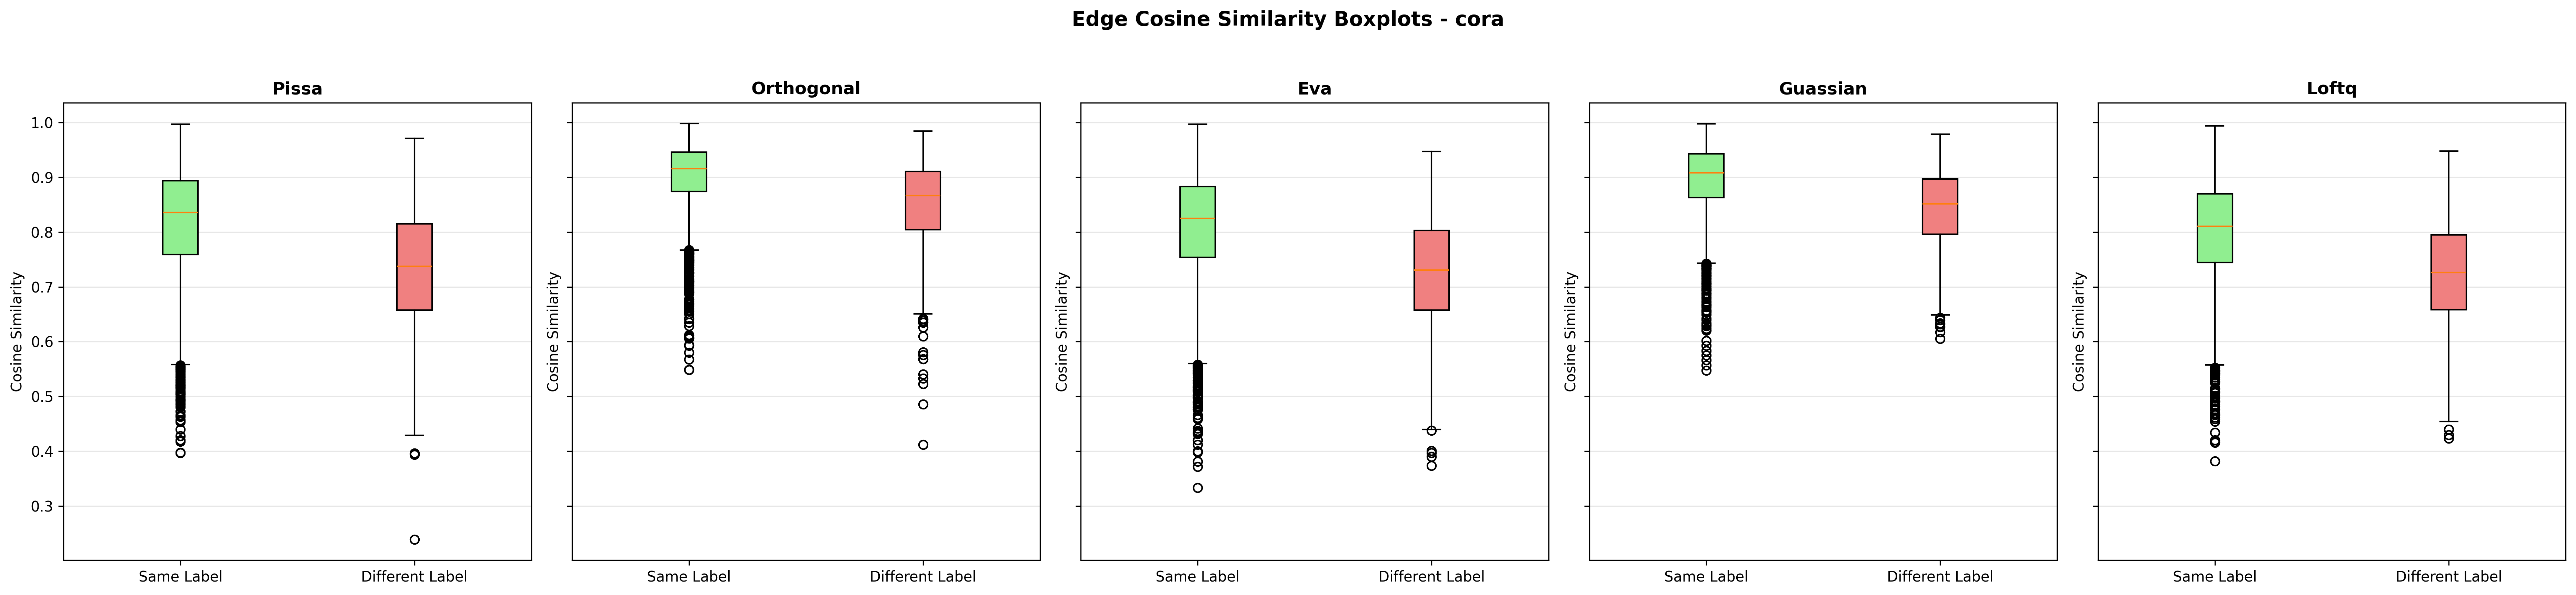
\includegraphics[width=1\textwidth]{Images/edge_similarity_boxplots_cora.png}
\caption{Boxplot of cosine similarity distributions for edges connecting nodes with identical and different labels}
\label{fig:cosine_box_plot}
\end{figure}

In this experiment, to examine the degree of alignment between the extracted semantic representations and the graph structure, cosine similarity between the representation vectors of the nodes at both ends of each edge was computed. This evaluation was performed separately for edges connecting same-label and different-label nodes. Table \ref{tab:mean_std_cos_similarity} reports the mean and standard deviation of cosine similarity for different methods.

According to the results, in all methods, the average cosine similarity for same-label edges is significantly higher than that for different-label edges. This difference indicates that the extracted semantic representations are able to properly distinguish same-class nodes from different-class nodes and are consistent with the homophily assumption of graphs.

On the other hand, the higher standard deviation in different-label edges indicates greater dispersion of semantic similarities in this group. This suggests the presence of edges whose endpoints, despite having different labels, still exhibit relatively high semantic similarity; an issue that may arise from structural noise or limitations of the original graph.

Figure \ref{fig:cosine_box_plot} also shows the distribution of these values using a box plot. As can be observed, the median and quartiles of cosine similarity for same-label edges are noticeably higher than those for different-label edges. This distributional separation provides a suitable basis for defining a threshold to identify and remove noisy edges.

Accordingly, it can be concluded that cosine similarity in the rich representation space extracted from large language models is an effective criterion for detecting invalid edges in the graph. Removing these edges increases structural homophily and provides a more suitable foundation for training graph neural networks.

\subsection{Sensitivity analysis of the model with respect to the cosine similarity threshold}

\begin{figure}[ht]
\begin{subfigure}{0.3\linewidth}
  \centering
  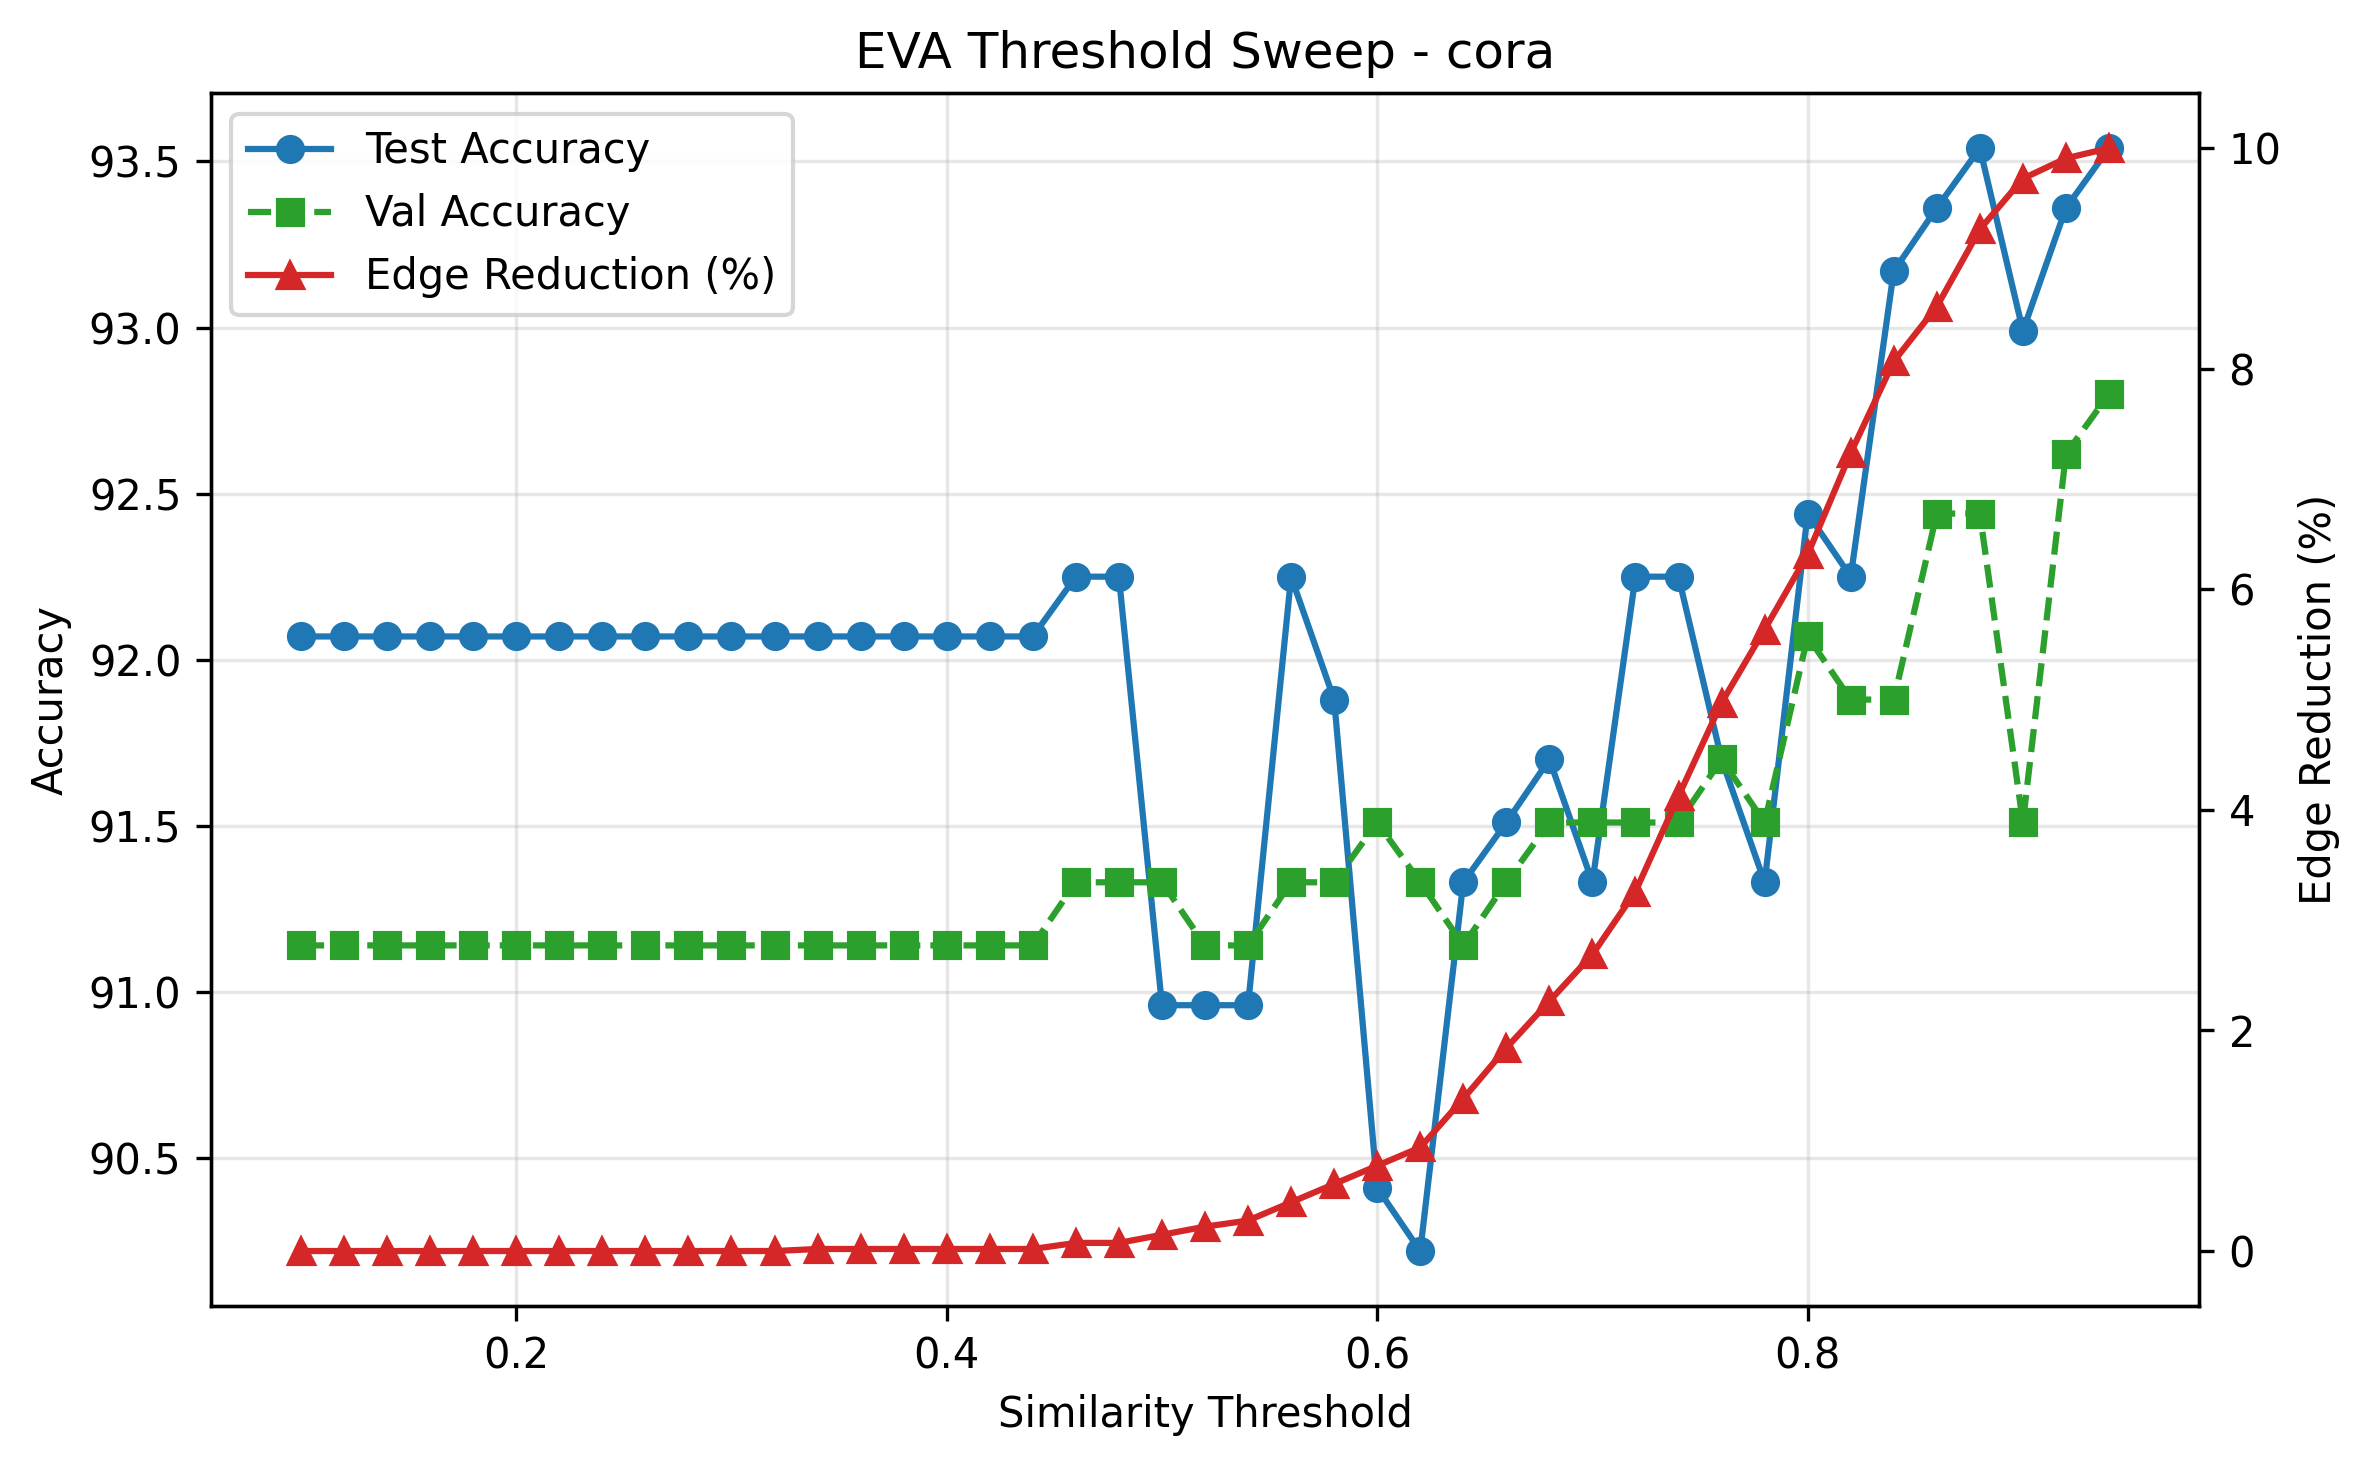
\includegraphics[width=\linewidth]{Images/threshold_analysis_eva_cora.png}
  \caption{EVA}
\end{subfigure}
\hfill
\begin{subfigure}{0.3\linewidth}
  \centering
  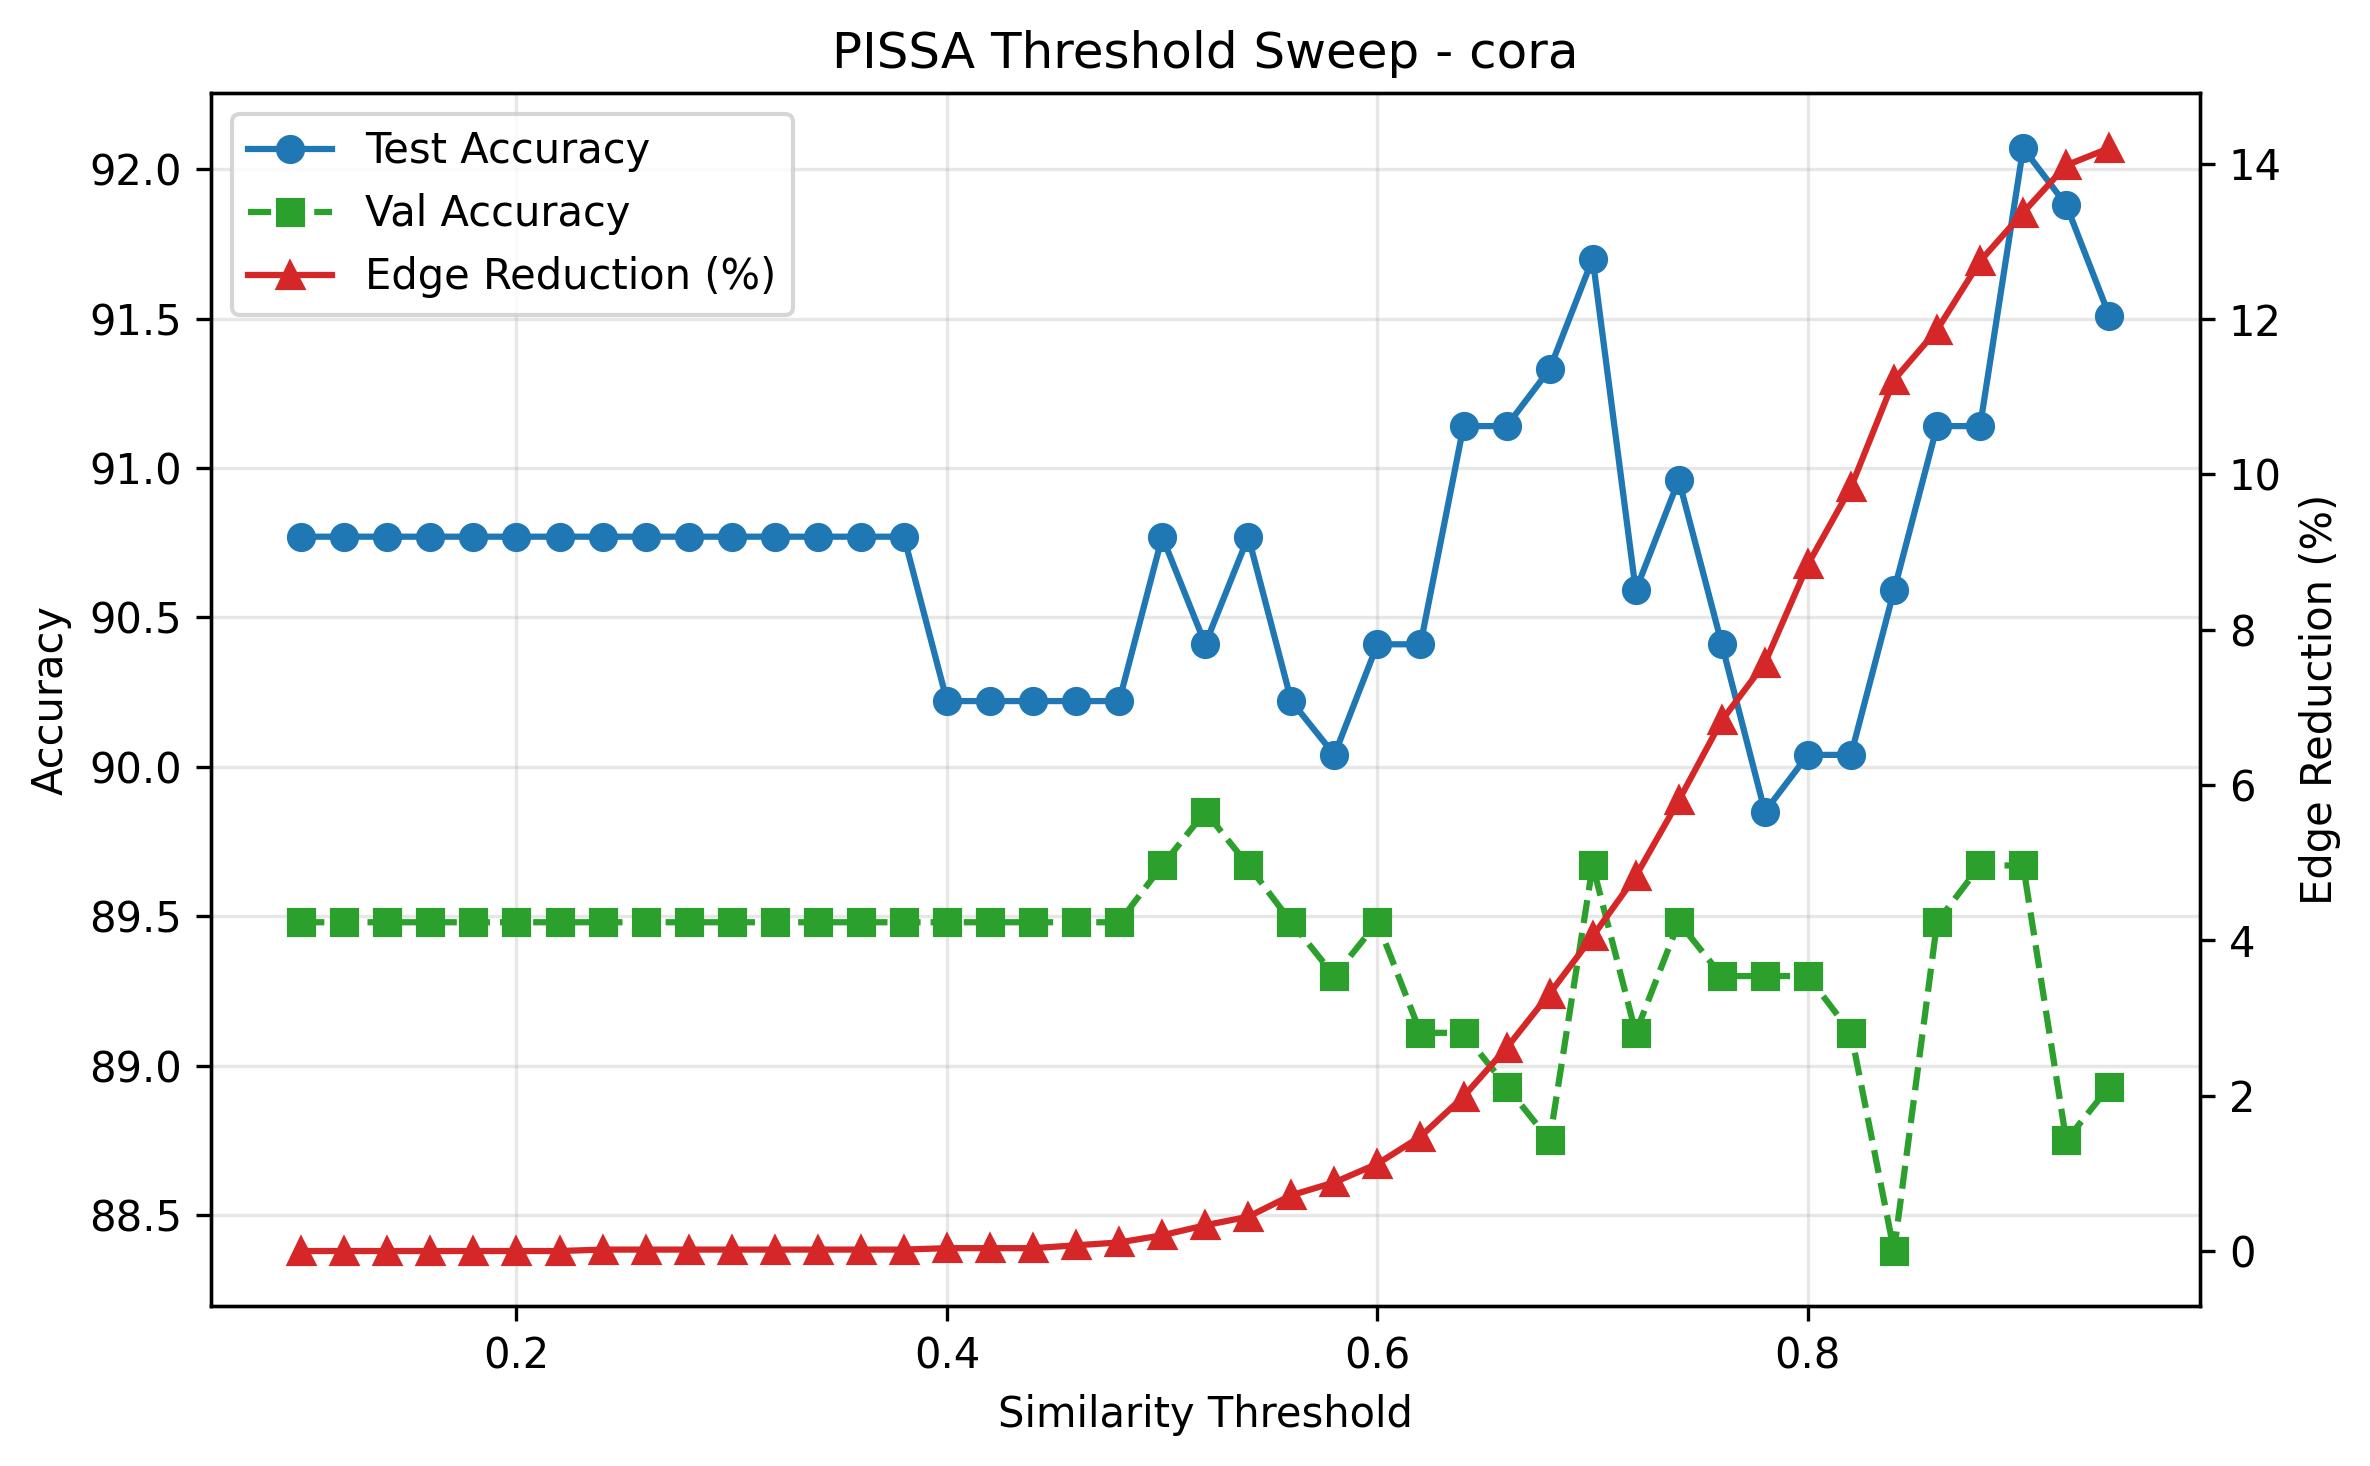
\includegraphics[width=\linewidth]{Images/threshold_analysis_pissa_cora.png}
  \caption{PiSSA}
\end{subfigure}
\hfill
\begin{subfigure}{0.3\linewidth}
  \centering
  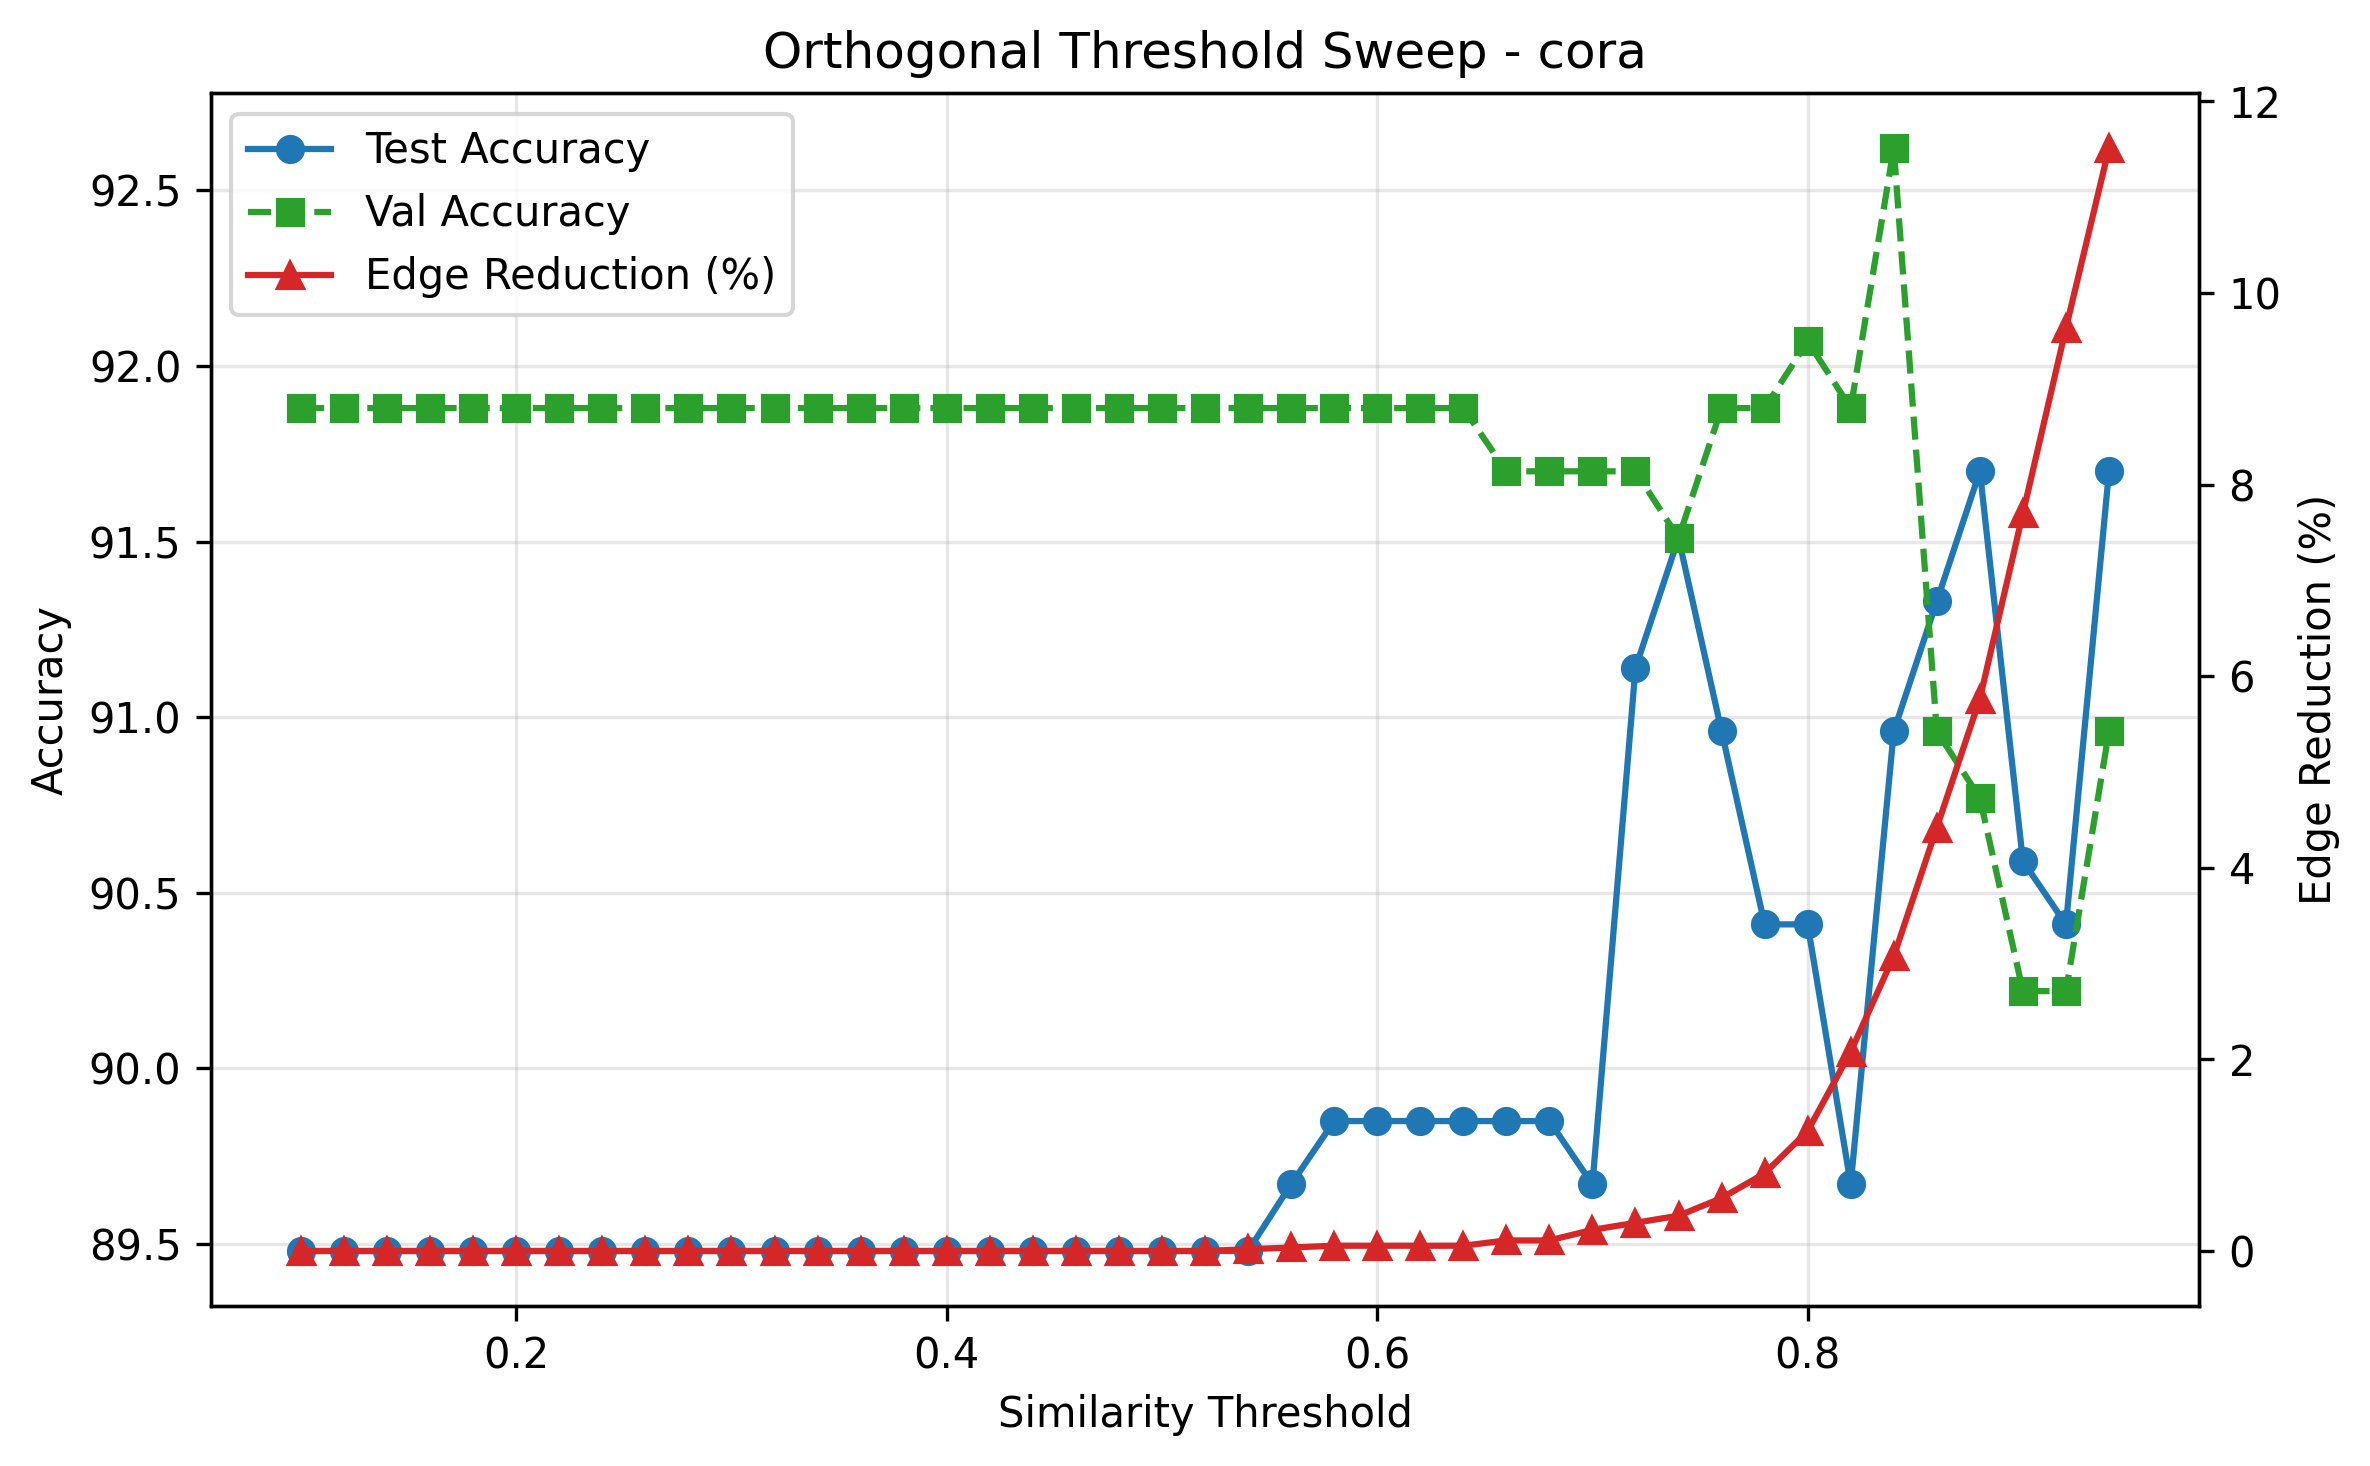
\includegraphics[width=\linewidth]{Images/threshold_analysis_orthogonal_cora.png}
  \caption{Orthogonal}
\end{subfigure}
\begin{subfigure}{0.3\linewidth}
  \centering
  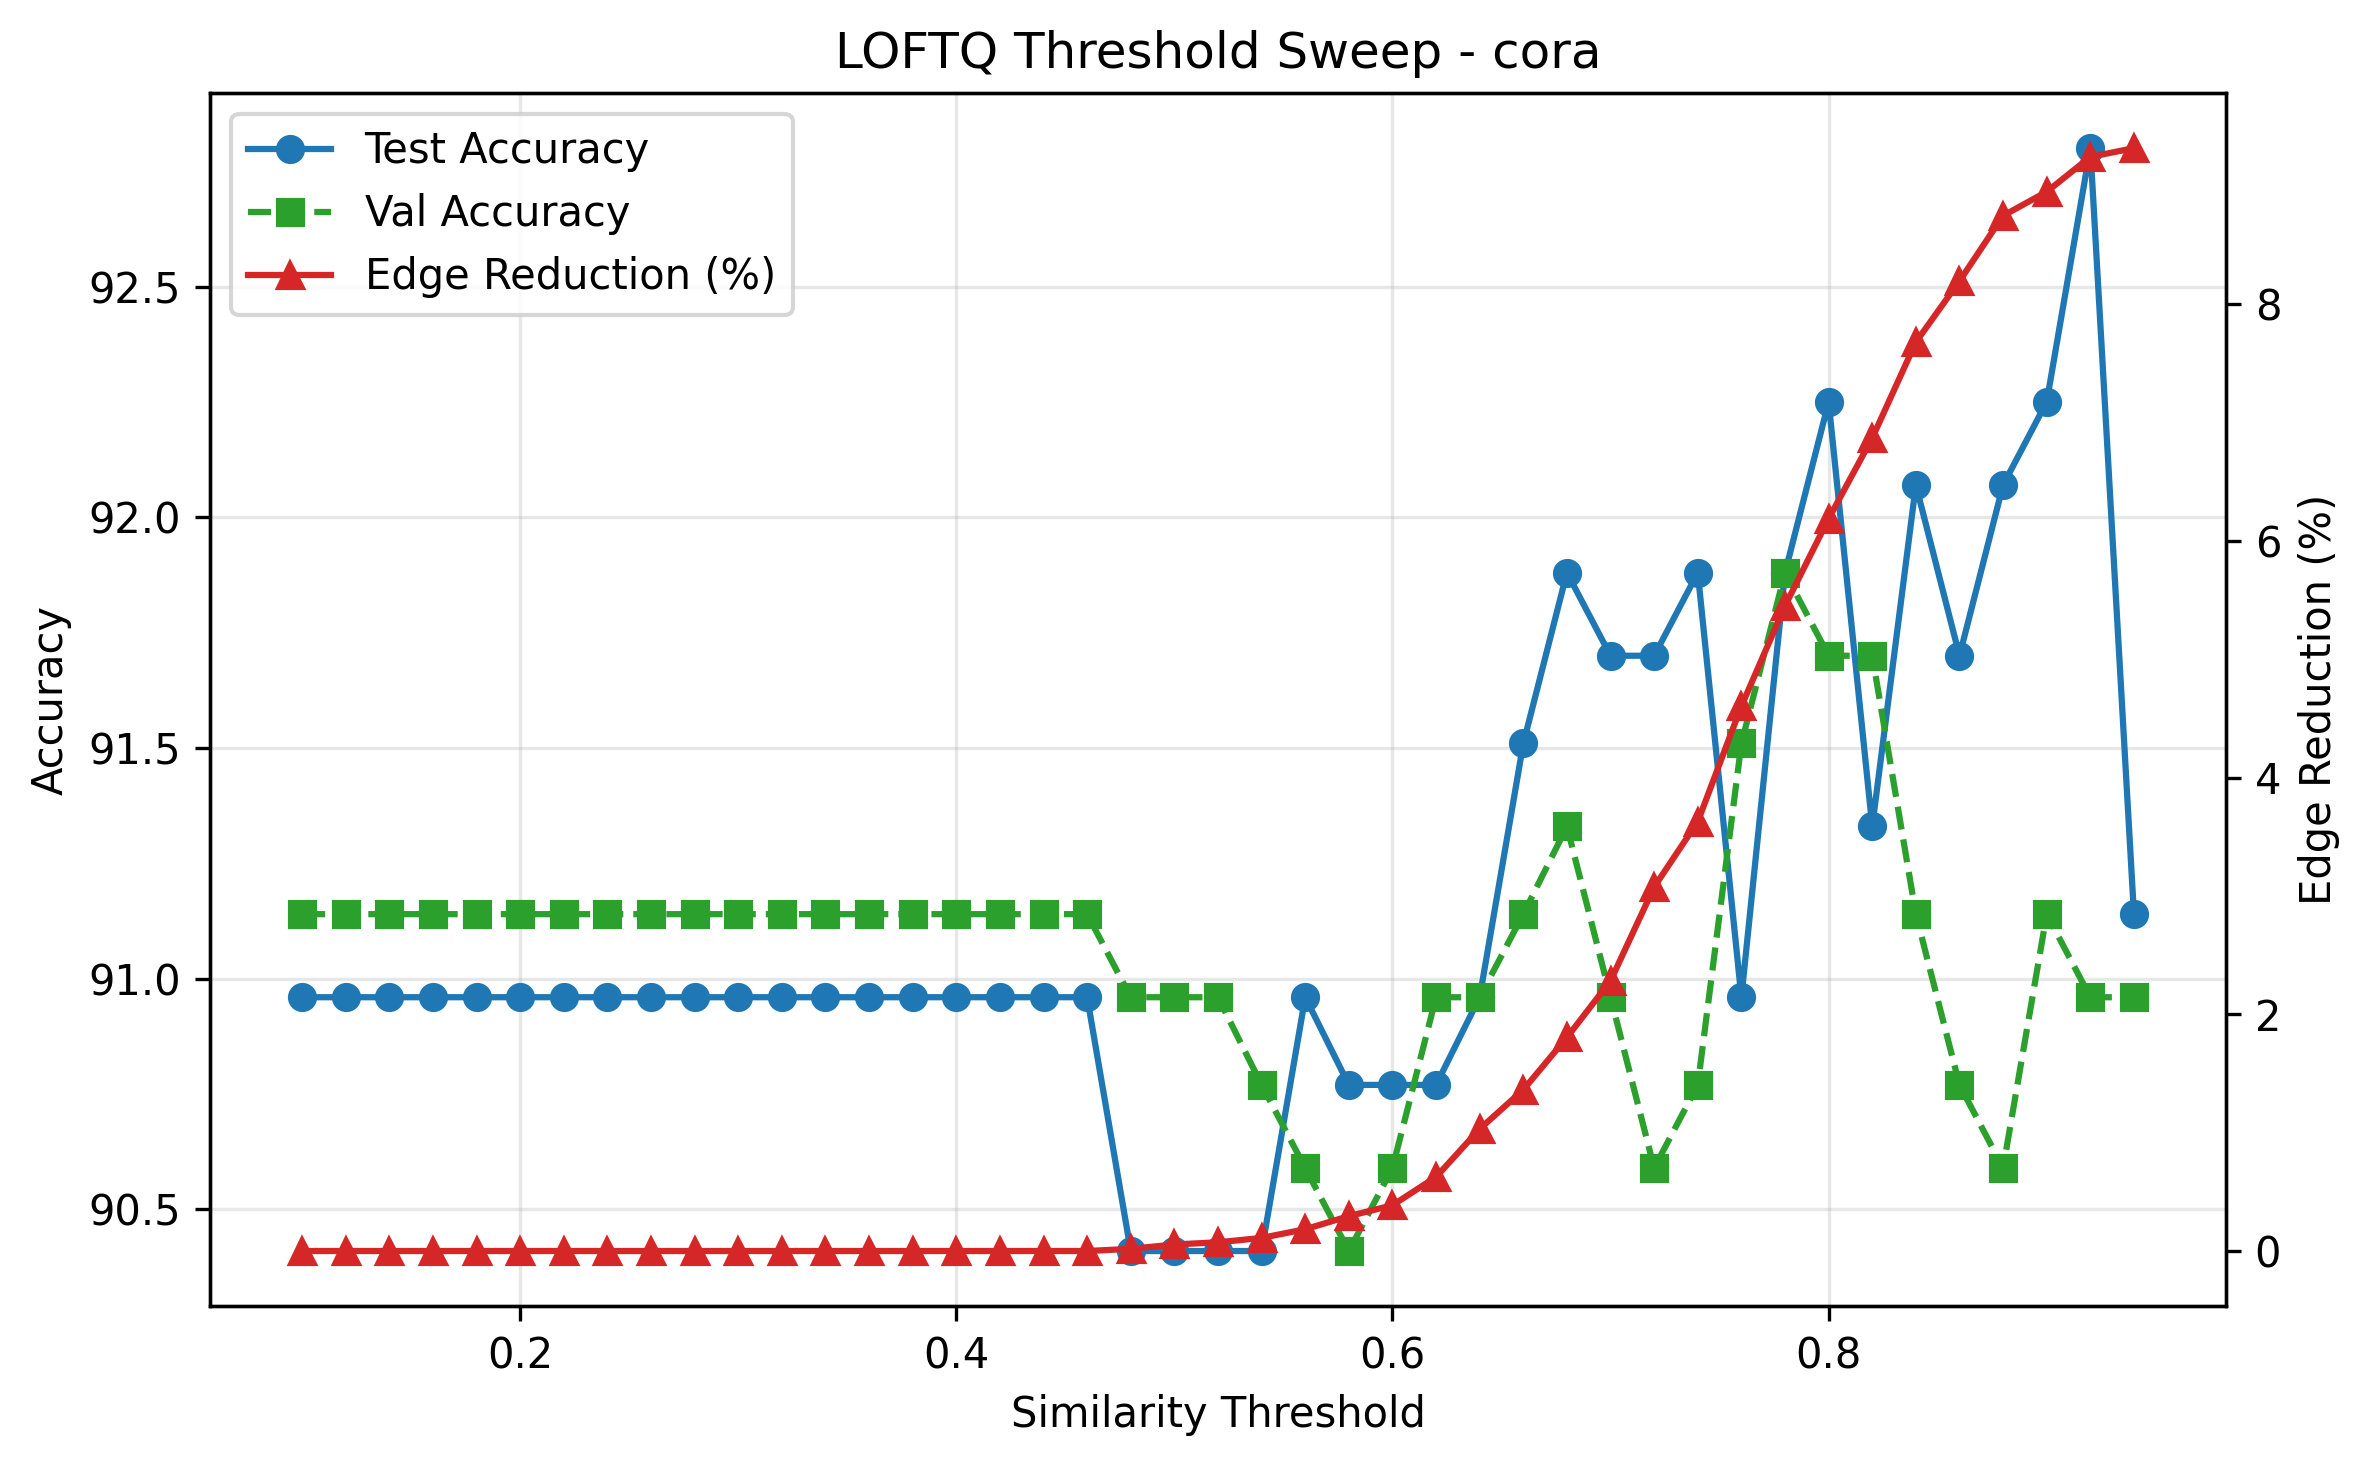
\includegraphics[width=\linewidth]{Images/threshold_analysis_loftq_cora.png}
  \caption{LoFTQ}
\end{subfigure}
\begin{subfigure}{0.3\linewidth}
  \centering
  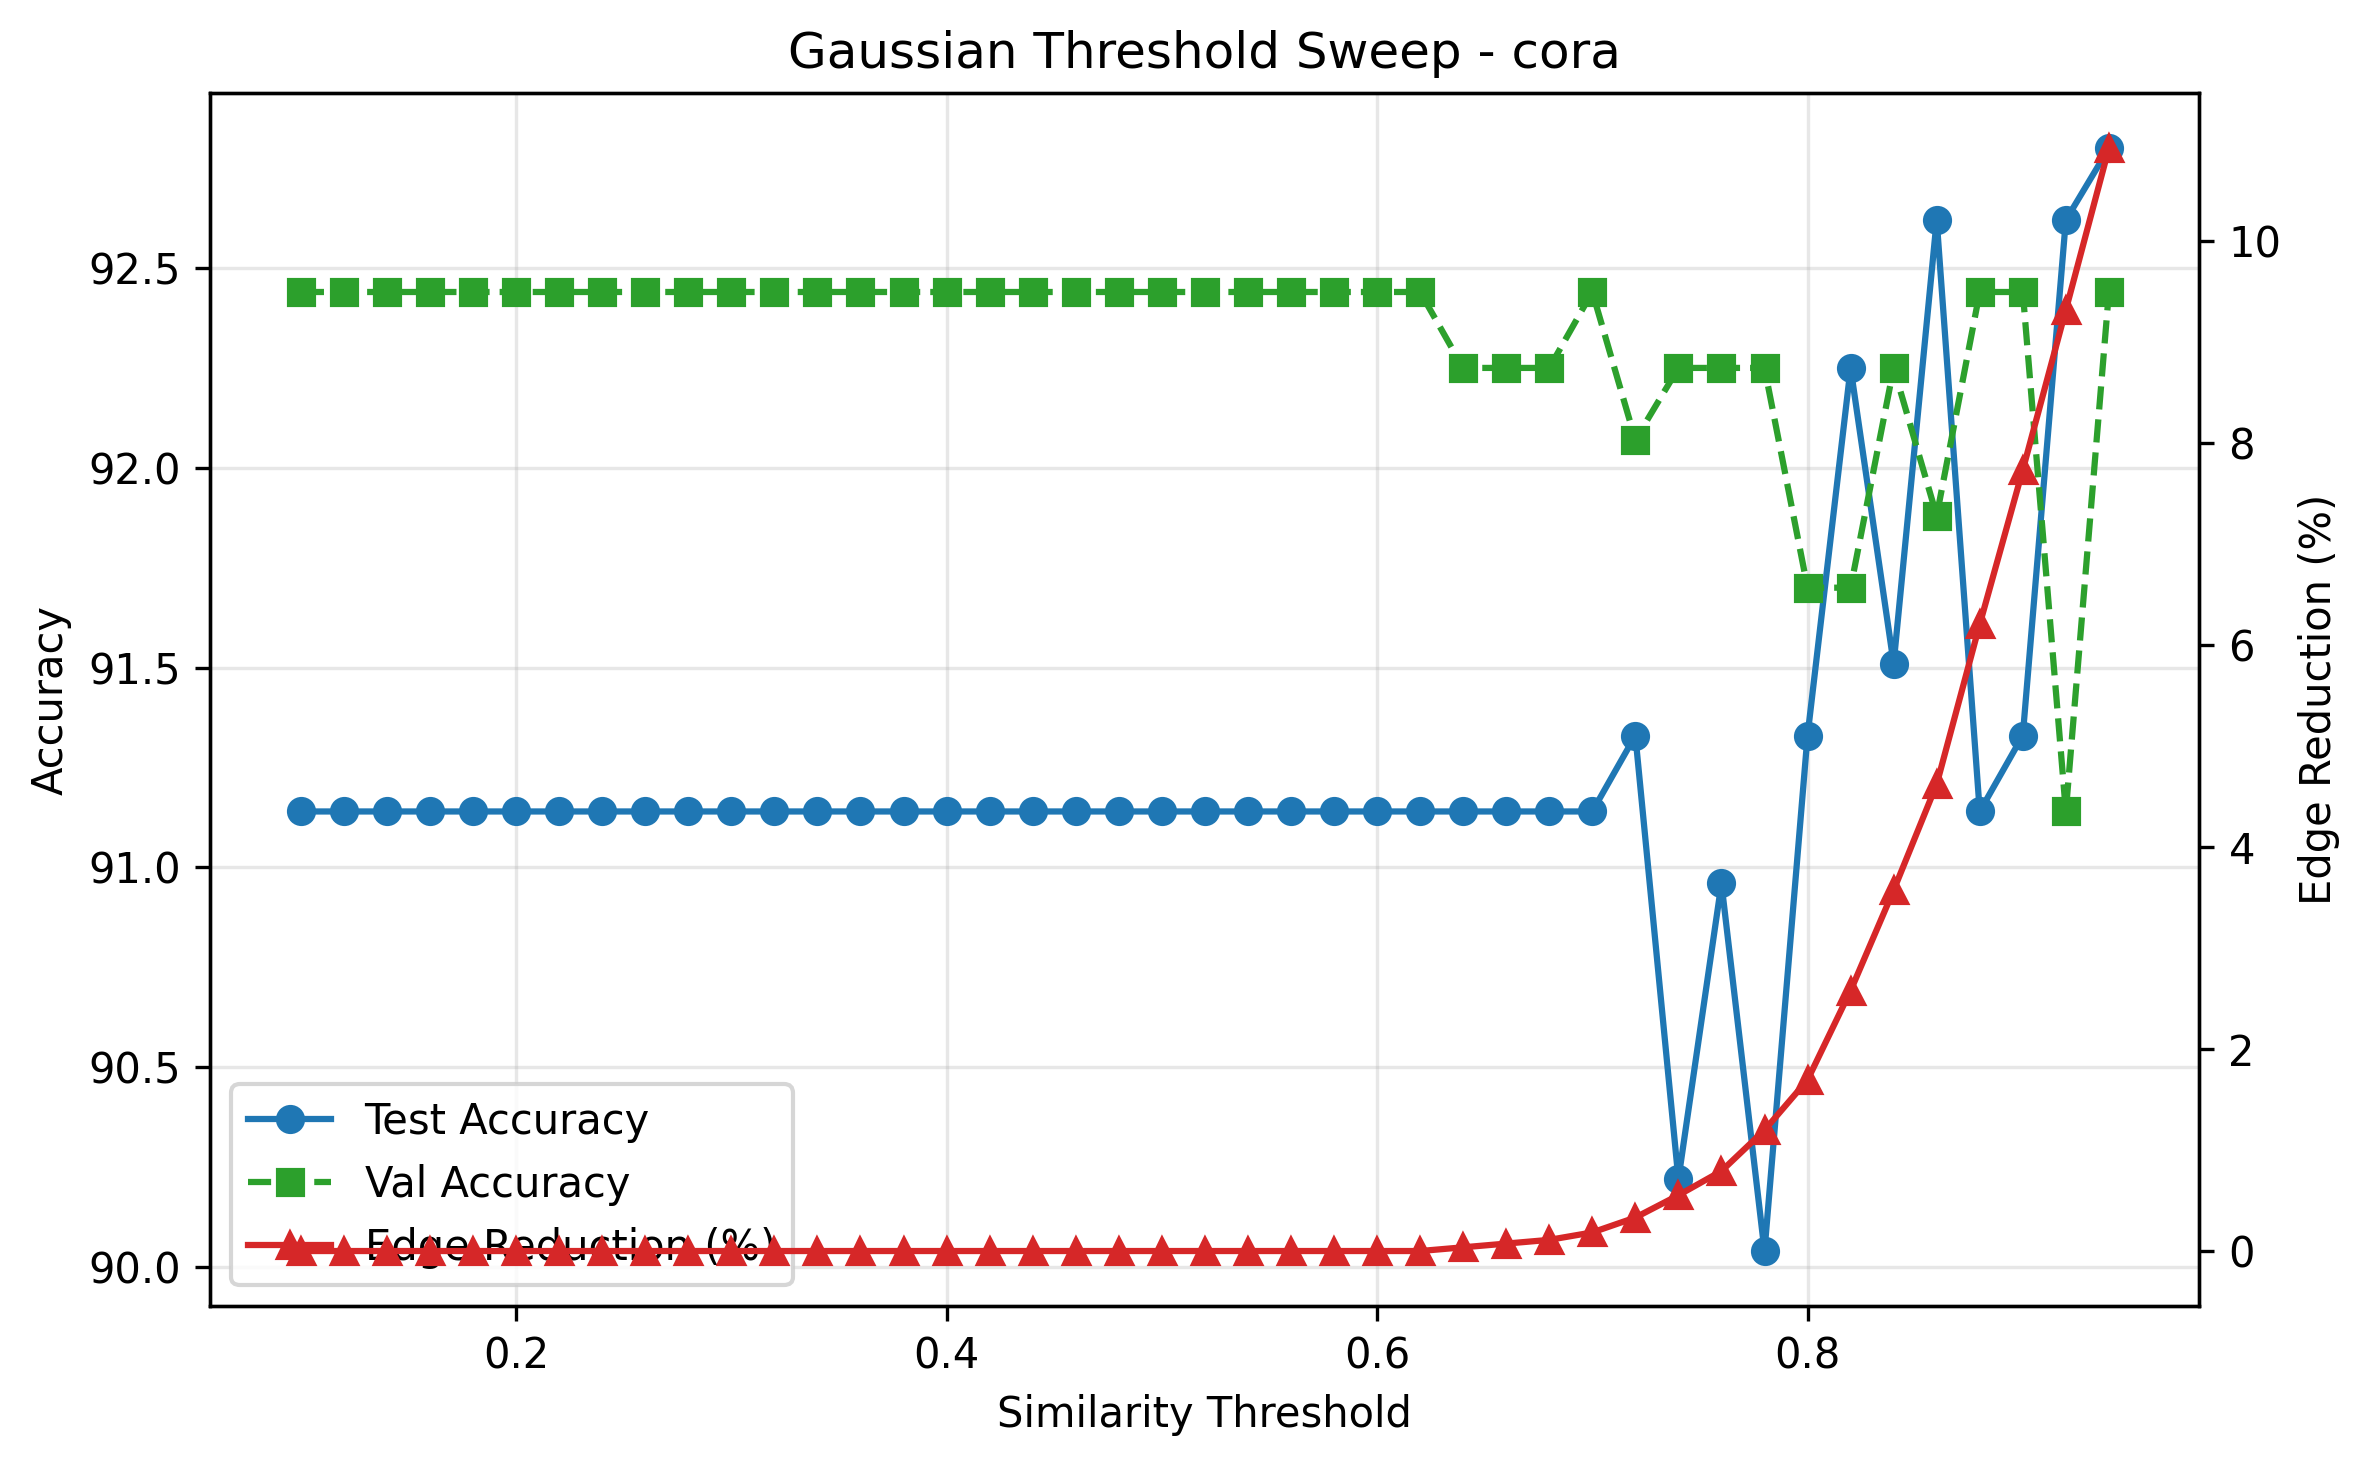
\includegraphics[width=\linewidth]{Images/threshold_analysis_gaussian_cora.png}
  \caption{Gaussian}
\end{subfigure}
\centering
\caption{
Changes in model accuracy as a function of the percentage of removed edges
for different values of the cosine similarity threshold
across different textual representations on the Cora dataset
}
\label{fig:multi}
\end{figure}

In this section, the effect of the cosine similarity threshold on model performance and the degree of graph structure refinement is investigated. The results of this analysis for different textual representations are presented in Figure \ref{fig:multi}.

The results show that at low threshold values, the percentage of removed edges is approximately zero, and the graph structure essentially remains unchanged. In this region, model accuracy is also nearly constant, indicating the negligible effect of graph refinement when very conservative thresholds are used.

With a gradual increase in the threshold value, the process of removing noisy edges becomes active, and the percentage of removed edges increases in a nonlinear manner. For most representations, especially EVA and Gaussian, a mid-range interval of threshold values is observed in which, despite a limited increase in the percentage of removed edges, model accuracy not only does not decrease but even improves in some cases. This behavior indicates that removing edges with low semantic similarity can increase graph homophily and improve the message-passing process in graph neural networks.

At higher threshold values, with a sharp increase in the percentage of removed edges, greater fluctuations in model accuracy are observed. This phenomenon is particularly evident in methods such as Orthogonal and PiSSA, and may be caused by excessive edge removal and the weakening of graph connectivity. In this situation, although graph refinement is performed more strongly, excessive reduction of structural information can have a negative effect on model performance.

Overall, the results of this experiment show that selecting the cosine similarity threshold plays a crucial role in balancing the reduction of structural noise and the preservation of useful graph information. The existence of an optimal threshold region, in which a suitable proportion of noisy edges is removed while model performance improves, confirms the necessity of performing this sensitivity analysis and carefully tuning this parameter in the proposed method.

\subsection{Comparison of Performance Before and After Cosine Similarity-Based Graph Refinement}

\begin{table}[ht]
\centering
\caption{Comparison of graph neural network model accuracy before and after cosine similarity-based graph structure refinement}
\label{tab:changing_after_cosine_enhancer_gnns_percentage}
\begin{tabularx}{\linewidth}{c c || *{5}{X}}
\hline
\multirow{2}{*}{Dataset} &
\multirow{2}{*}{Approach} &
\multicolumn{5}{c}{Method} \\
\cline{3-7}
 &  & PiSSA & Orthogonal & EVA & Gaussian & LoFTQ \\
\hline
\multirow{3}{*}{Cora}
 & before
 & 90.77 & 89.48 & 92.07 & 91.14 & 90.96 \\
\cline{2-7}
 & after
 & 90.77 & 90.41 & 92.07 & 90.04 & 91.88 \\
\cline{2-7}
 & improvement
 & 0.00 & +0.93 & 0.00 & -1.10 & +0.92 \\
\hline
\hline
\multirow{3}{*}{PubMed}
 & before
 & 96.32 & 93.79 & 96.96 & 94.80 & 96.17 \\
\cline{2-7}
 & after
 & 96.81 & 93.86 & 96.96 & 94.80 & 96.75 \\
\cline{2-7}
 & improvement
 & +0.49 & +0.07 & 0.00 & 0.00 & +0.58 \\
\hline
\hline
\multirow{3}{*}{CiteSeer}
 & before
 & 80.25 & 80.25 & 79.47 & 81.03 & 80.41 \\
\cline{2-7}
 & after
 & 80.25 & 81.97 & 79.15 & 81.03 & 79.78 \\
\cline{2-7}
 & improvement
 & 0.00 & +1.72 & -0.32 & 0.00 & -0.63 \\
\hline
\hline
\multirow{3}{*}{WikiCS}
 & before
 & 87.14 & 85.35 & 87.27 & 86.80 & 87.74 \\
\cline{2-7}
 & after
 & 88.12 & 85.48 & 88.64 & 87.01 & 89.06 \\
\cline{2-7}
 & improvement
 & +0.98 & +0.13 & +1.37 & +0.21 & +1.32 \\
\hline
\end{tabularx}
\end{table}


\begin{table}[ht]
\centering
\caption{Comparison of ensemble learning methods before and after cosine similarity-based graph refinement}
\label{tab:changing_after_cosine_enhancer_ensembles}
\begin{tabularx}{\linewidth}{| c|| c | X | X | X|}
\hline
Dataset & Ensemble & Before (\%) & After (\%) & Improvement (\%) \\
\hline
\multirow{3}{*}{PubMed}
 & Ensemble1 & 96.98 & 97.03 & +0.05 \\
 & Ensemble2 & 97.13 & 97.11 & -0.02 \\
 & Ensemble3 & 97.16 & 97.13 & -0.03 \\
\hline
\hline
\multirow{3}{*}{CiteSeer}
 & Ensemble1 & 81.66 & 81.03 & -0.63 \\
 & Ensemble2 & 81.97 & 81.82 & -0.15 \\
 & Ensemble3 & 82.13 & 81.50 & -0.63 \\
\hline
\hline
\multirow{3}{*}{WikiCS}
 & Ensemble1 & 88.34 & 88.72 & +0.38 \\
 & Ensemble2 & 88.38 & 89.19 & +0.81 \\
 & Ensemble3 & 88.42 & 89.28 & \textbf{+0.86} \\
\hline
\hline
\multirow{3}{*}{Cora}
 & Ensemble1 & 93.17 & 93.91 & +0.74 \\
 & Ensemble2 & 93.36 & 94.10 & +0.74 \\
 & Ensemble3 & 93.17 & 94.10 & \textbf{+0.93} \\
\hline
\end{tabularx}
\end{table}

In Table \ref{tab:changing_after_cosine_enhancer_gnns_percentage},
the performance of graph neural networks before and after cosine similarity-based graph refinement is compared.
As can be observed,
in most representations and datasets,
structural refinement leads to improved accuracy.
These results indicate that removing edges with low semantic similarity
can reduce structural noise
and improve the quality of local neighborhoods.

Table \ref{tab:changing_after_cosine_enhancer_ensembles}
also compares the performance of ensemble learning methods
under before and after graph refinement conditions.
In most cases,
applying refinement leads to improved ensemble performance,
which indicates the complementarity of graph structural enhancement
and textual representation diversity within the proposed framework.

It is also observed that in datasets with a higher edge-to-node ratio,
the effect of structural refinement is more pronounced.
In denser graphs,
the likelihood of noisy edges is higher,
and their targeted removal can
lead to increased homophily and improved message passing in graph neural networks.

As an example,
in the WikiCS dataset,
which has higher density compared to other datasets,
a more significant increase in accuracy is observed.
This finding suggests that the effectiveness of semantic similarity-based refinement
also depends on the structural characteristics of the graph.

\subsection{Evaluation and Comparison with State-of-the-Art Methods}

\begin{table}[htbp]
\centering
\caption{
Comparison of the accuracy of the proposed method DIVERGE with cosine similarity-based structural enhancement
against previous methods
}
\label{tab:diverge_with_cosine_enhancer_ensembles_accuracy}
\begin{tabularx}{\textwidth}{l|X|X|X|X}
\hline
\diagbox[dir=NE, outerrightsep=40pt]{\textbf{Dataset (\%)}}{\textbf{Method}} & Cora & CiteSeer & PubMed & WikiCS \\
\hline
\hline
GCN & 87.41 & 75.74 & 89.01 & 83.67 \\
SAGE & 87.44 & 74.96 & 90.47 & 84.86 \\
GAT & 86.68 & 73.73 & 88.25 & 83.94 \\
SenBERT-66M & 79.61 & 74.06 & 94.47 & 86.51  \\
RoBERTa-355M & 83.17 & 75.90 & 94.84 & 87.47 \\
ENGINE & 87.00 & 75.82 & 90.08 & 85.44  \\
TAPE & 90.05 & 76.45 & 93.00 & 87.11  \\
GraphGPT & 82.29 & 74.67 & 93.54 & 82.54  \\
LLaGA & 87.55 & 76.73 & 90.28 & 84.03  \\
\hline
\hline
DIVERGE 1 + Semantic Structure Enhancer & \textbf{93.91} & \textbf{81.03} & \textbf{97.03} & \textbf{89.32}  \\
DIVERGE 2 + Semantic Structure Enhancer & \textbf{94.10} & \textbf{81.82} & \textbf{97.11} & \textbf{89.19} \\
DIVERGE 3 + Semantic Structure Enhancer & \textbf{94.10} & \textbf{81.50} & \textbf{97.13} & \textbf{89.28} \\
\hline
\hline
\end{tabularx}
\end{table}



\begin{table}[htbp]
\centering
\caption{
Comparison of Macro-F1 scores for previous methods
and different versions of DIVERGE with graph structure refinement
}
\label{tab:diverge_with_cosine_enhancer_ensembles_accuracy_macro_f1}
\begin{tabularx}{\textwidth}{l|X|X|X|X}
\hline
\diagbox[dir=NE, outerrightsep=40pt]{\textbf{Dataset (\%)}}{\textbf{Method}} 
& Cora & CiteSeer & PubMed & WikiCS \\
\hline
\hline
GCN & 86.54 & 71.52 & 88.54 & 82.11\\
SAGE & 86.37 & 71.87 & 90.16 & 82.78 \\
GAT & 85.64 & 69.27 & 87.70 & 82.14 \\
SenBERT-66M & 77.13 & 71.25 & 93.95 & 84.43 \\
RoBERTa-355M & 81.38 & 72.31 & 94.33 & 86.01  \\
ENGINE & 85.72 & 71.22 & 89.63 & 83.80  \\
TAPE & 87.21 & 73.33 & 92.39 & 86.03  \\
GraphGPT & 74.08 & 61.04 & 90.89 & 73.92 \\
LLaGA & 84.97 & 72.59 & 90.00 & 82.37  \\
\hline
\hline
DIVERGE 1 + Semantic Structure Enhancer 
& \textbf{92.65} & \textbf{77.92} & \textbf{96.60} & \textbf{88.43} \\
DIVERGE 2 + Semantic Structure Enhancer 
& \textbf{92.99} & \textbf{78.56} & \textbf{96.74} & \textbf{88.27} \\
DIVERGE 3 + Semantic Structure Enhancer 
& \textbf{92.96} & \textbf{78.37} & \textbf{96.77} & \textbf{88.09} \\
\hline
\hline
\end{tabularx}
\end{table}

In Table \ref{tab:diverge_with_cosine_enhancer_ensembles_accuracy},
the performance of the proposed method DIVERGE with cosine similarity-based graph structural refinement
is reported in terms of accuracy.
In addition, Table \ref{tab:diverge_with_cosine_enhancer_ensembles_accuracy_macro_f1}
presents the comparison in terms of Macro-F1 score.

The results show that in the unrefined setting,
the proposed method achieves state-of-the-art performance across all datasets.
With the application of structural refinement,
further improvements are also observed in some datasets.
This finding indicates that graph structural enhancement
can act as a complementary mechanism for the DIVERGE framework
and, in some cases, push the performance beyond the state-of-the-art boundary.

\subsection{Evaluation of the Third Proposed Method: Uncertainty-Based Graph Structure Refinement for Edge Prediction}

In this method, similar to the previous approach, the goal is to refine the graph structure
and improve node classification performance by identifying and removing noisy edges.
However, in this case, instead of using semantic similarity or distance,
graph neural networks and extracted semantic representations are employed.

Within this framework, a graph neural network acts as an edge prediction model.
This model estimates the probability of the existence or absence of each edge in the graph
by taking as input the semantic representations produced by a large language model.
In other words, for each pair of nodes,
the likelihood of an edge between them is estimated.

To quantify uncertainty in the predictions,
the edge prediction model is retrained multiple times with different training samples.
As a result, a set of probability estimates is obtained for each edge.
Then, using entropy and standard deviation measures,
the uncertainty associated with each edge is computed.

Finally, based on the defined strategies,
edges with high uncertainty are identified as noisy edges and removed from the graph.
This graph refinement process
leads to a reduction in structural noise and ultimately improves model performance
in the node classification task.

\subsection{Comparison of Uncertainty Measures for Noisy Edge Detection}

\begin{figure}[h]
    \centering
    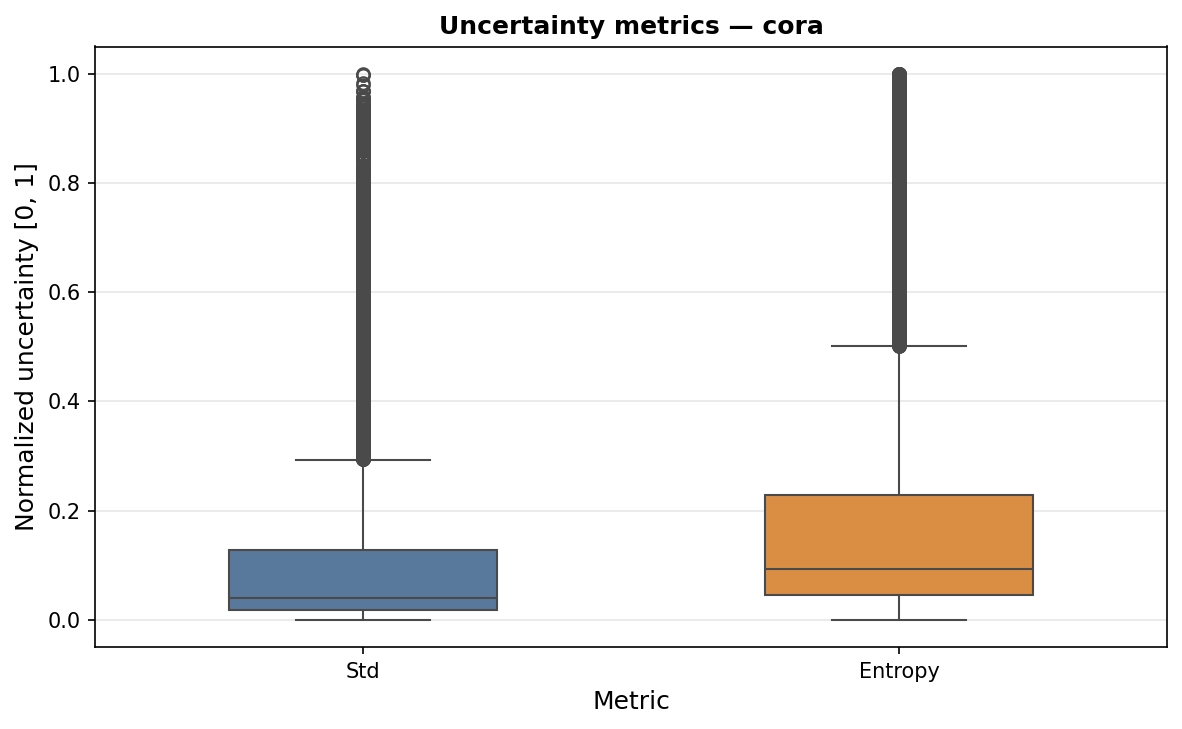
\includegraphics[width=0.5\textwidth]{Images/uncertainty_boxplot_seaborn_cora.png}
    \caption{Box plot of edge uncertainty distribution based on entropy and standard deviation}
    \label{fig:edge_similarity_boxplots_cora}
\end{figure}

In this experiment, to estimate edge prediction uncertainty in the Cora dataset,
multiple edge prediction models were trained using bootstrap sampling;
in each training run, a different subset of the data was selected,
and an independent model was learned.
Then, for each edge, the variability of model outputs was computed,
and two measures, standard deviation and entropy, were extracted as uncertainty indicators.

The box plot in Figure \ref{fig:edge_similarity_boxplots_cora}
shows that uncertainty based on the entropy measure
is generally larger and more dispersed than that of standard deviation.
The median and interquartile range of entropy are higher,
and more outliers are also observed,
indicating the higher sensitivity of this measure to variations in model predictions.

In contrast, standard deviation tends to have smaller values for most edges
and is concentrated near zero;
therefore, it mainly reflects the numerical stability of predictions,
while entropy provides a more comprehensive view of the level of uncertainty across models.

\subsection{Evaluation of Edge Removal Strategy Based on Thresholding}

\begin{figure}[h]
    \centering
    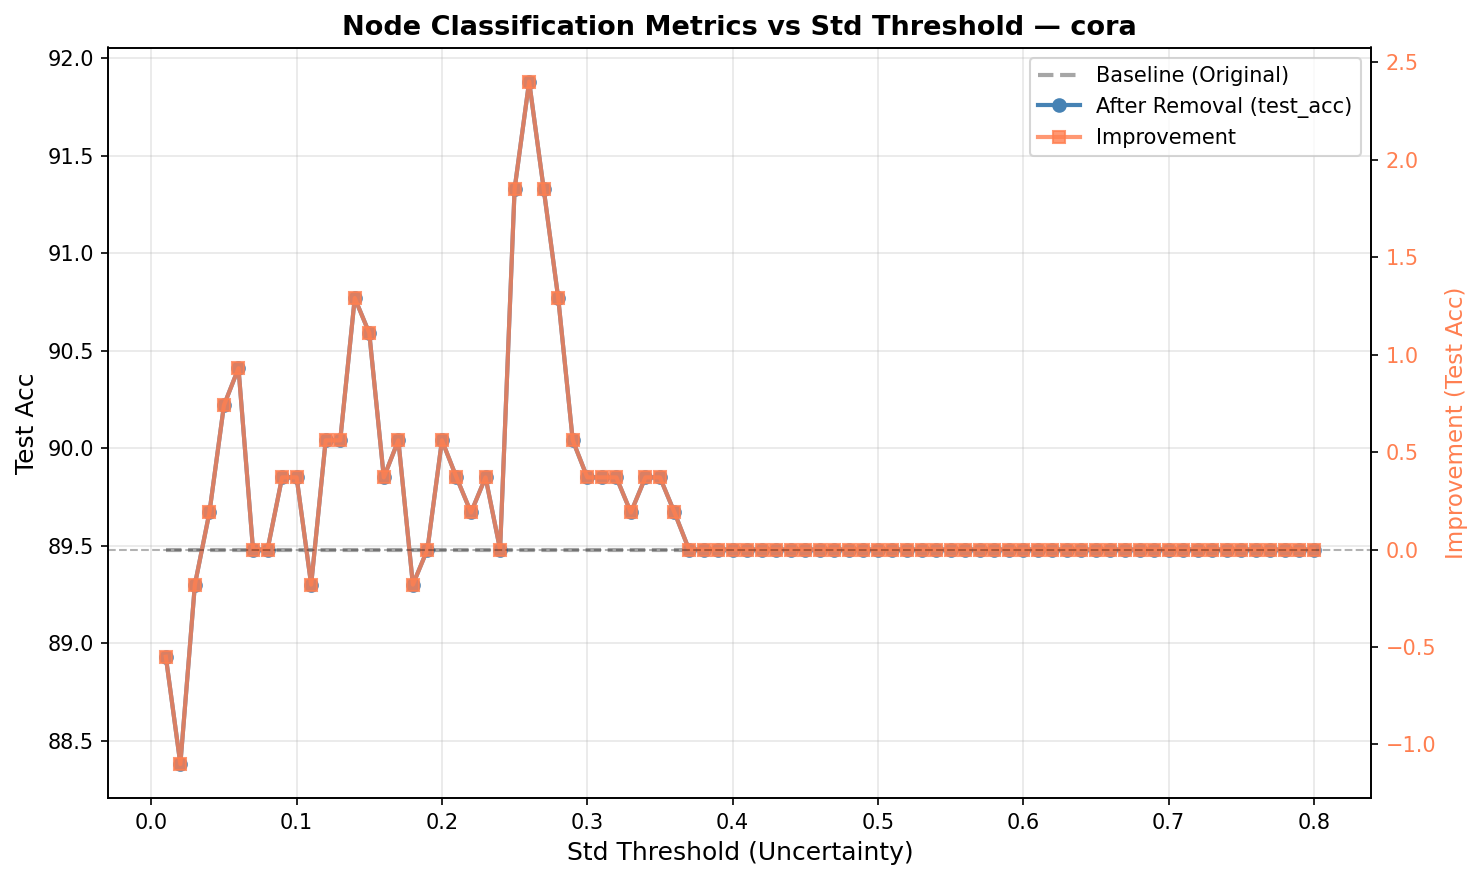
\includegraphics[width=0.5\textwidth]{Images/line_plot_combined_testacc_std_threshold_cora.png}
\caption{
Comparison of different threshold values for detecting noisy edges
based on the uncertainty measure of standard deviation
and model accuracy in node classification after graph refinement
}
    \label{fig:line_plot_combined_testacc_std_threshold_cora}
\end{figure}

\begin{figure}[h]
    \centering
    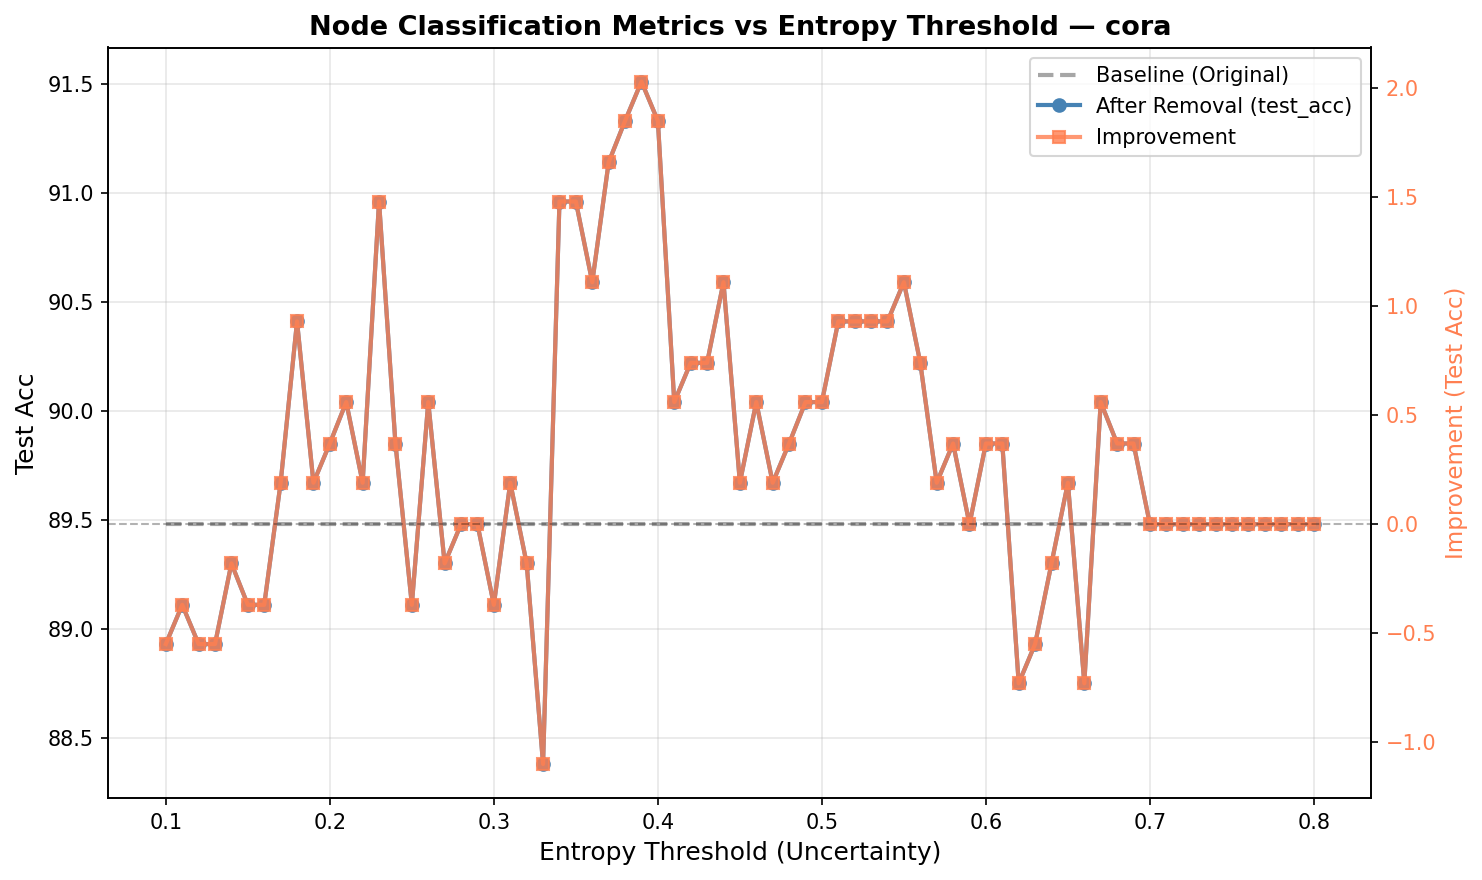
\includegraphics[width=0.5\textwidth]{Images/line_plot_combined_testacc_entropy_threshold_cora.png}
    \caption{
    Comparison of different threshold values for detecting noisy edges
    based on the uncertainty measure of entropy
    and model accuracy in node classification after graph refinement
    }
    \label{fig:line_plot_combined_testacc_entropy_threshold_cora}
\end{figure}

In this experiment, a thresholding strategy is used to identify
and remove noisy edges from the graph.
In this approach, different threshold values are compared with the uncertainty of each edge,
and if the uncertainty of an edge exceeds the defined threshold,
that edge is considered noisy and removed.

In the presented figures, two different measures are used to quantify uncertainty.
In Figure \ref{fig:line_plot_combined_testacc_std_threshold_cora},
standard deviation is used as the uncertainty indicator,
while in Figure \ref{fig:line_plot_combined_testacc_entropy_threshold_cora},
entropy is used as the uncertainty measure.
After removing noisy edges, the performance of the refined graph
is evaluated in the node classification task.
The vertical axis of the plots shows the accuracy of the trained graph neural network.

The results show that using standard deviation
in the threshold-based edge removal strategy
provides more stable behavior compared to entropy
and generally leads to improved classification performance across most threshold values.
It is also observed that as the threshold increases,
the number of edges identified as noisy decreases.
At higher threshold values,
almost no edges are removed;
as a result, the graph structure remains unchanged
and model performance becomes approximately constant beyond that point.

\subsection{Analysis of the Strategy for Removing a High Percentage of Most Uncertain Edges}

\begin{figure}[h]
    \centering
    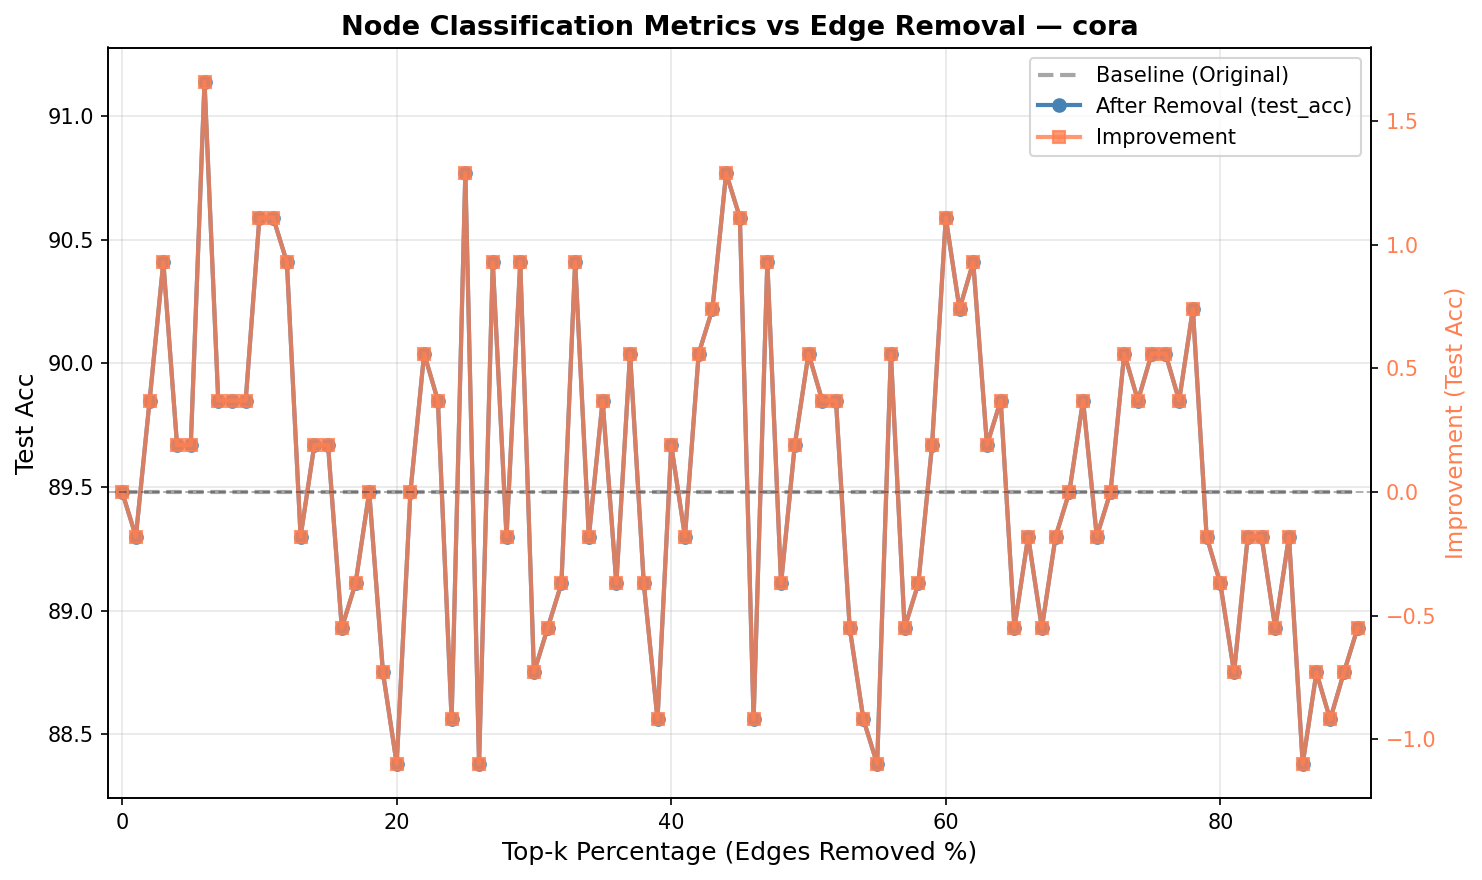
\includegraphics[width=0.5\textwidth]{Images/line_plot_combined_testacc_std_topk_cora.png}
\caption{
Comparison of removing a percentage of high-uncertainty edges based on the standard deviation measure
and its effect on node classification performance
}
    \label{fig:line_plot_combined_testacc_std_topk_cora}
\end{figure}

\begin{figure}[h]
    \centering
    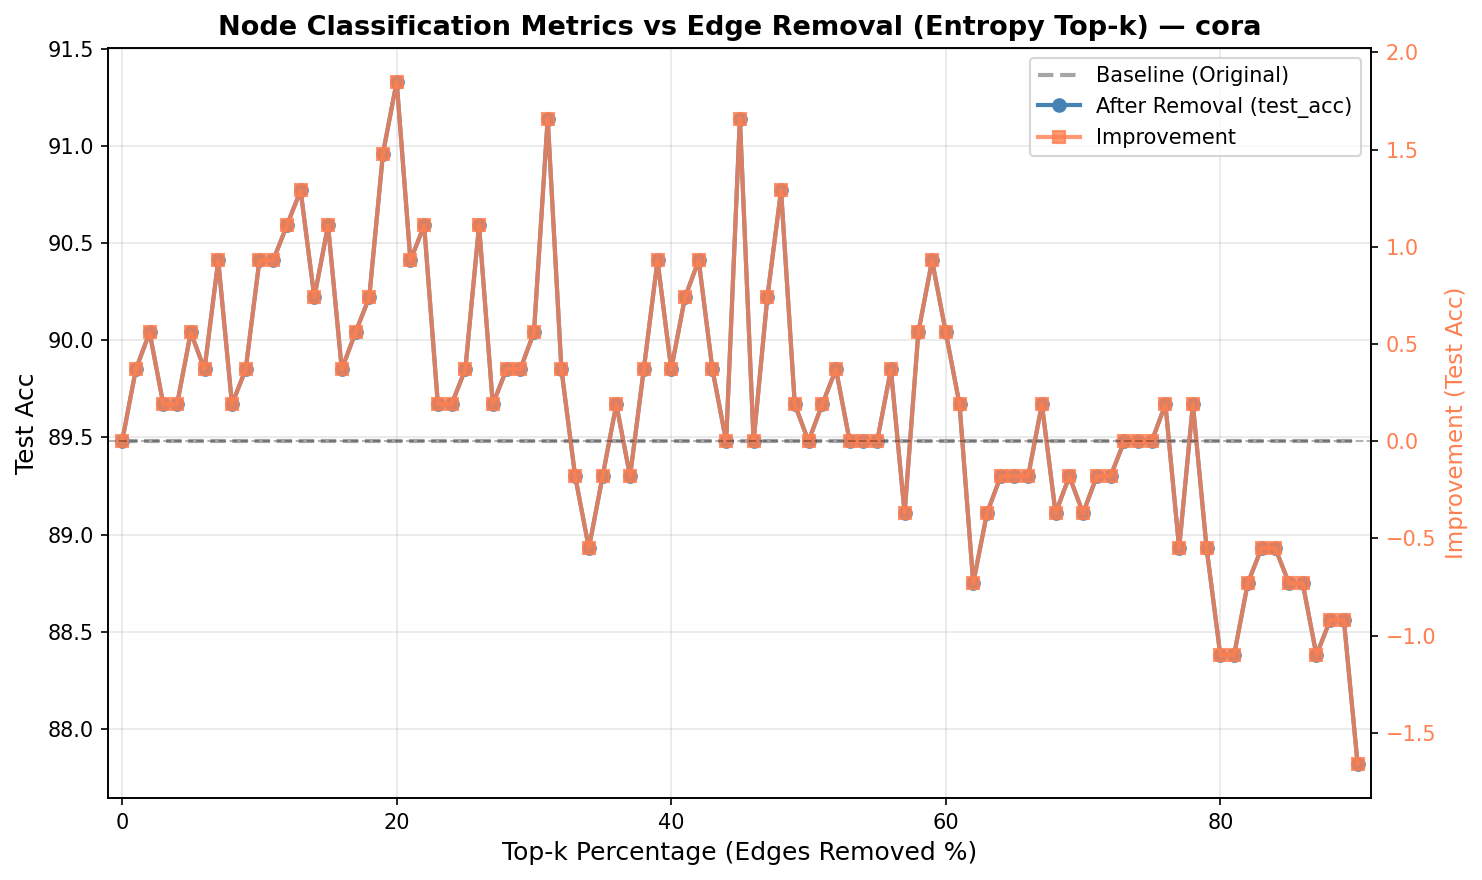
\includegraphics[width=0.5\textwidth]{Images/line_plot_combined_testacc_entropy_topk_cora.png}
\caption{
Comparison of removing a percentage of high-uncertainty edges based on the entropy measure
and its effect on node classification performance
}
    \label{fig:line_plot_combined_testacc_entropy_topk_cora}
\end{figure}

In this experiment, a top-k uncertainty-based edge removal strategy is used.
In this method, the top k percent of edges with the highest uncertainty values
are identified as noisy edges and removed from the graph.
In other words, instead of defining a fixed threshold,
a fixed percentage of the most uncertain edges is always removed.

In the corresponding figures, two different uncertainty measures are used.
In Figure \ref{fig:line_plot_combined_testacc_std_topk_cora},
standard deviation is used as the uncertainty metric,
while in Figure \ref{fig:line_plot_combined_testacc_entropy_topk_cora},
entropy is used.
In these plots, moving along the horizontal axis toward higher values
corresponds to removing a larger percentage of edges,
and thus leads to greater changes in the graph structure.

The results show that this strategy,
compared to the threshold-based strategy,
exhibits greater instability in performance.
It is also observed that when standard deviation is used as the uncertainty indicator,
changes in the percentage of removed edges introduce higher fluctuations in accuracy,
and the model shows greater sensitivity to these changes.
In contrast, using entropy in this strategy
leads to more stable performance
and provides better overall robustness.

```latex id="x7k3pm"
\subsection{Investigation of the Effect of the Number of Edge Prediction Models on Noisy Edge Detection}

\begin{figure}[h]
    \centering
    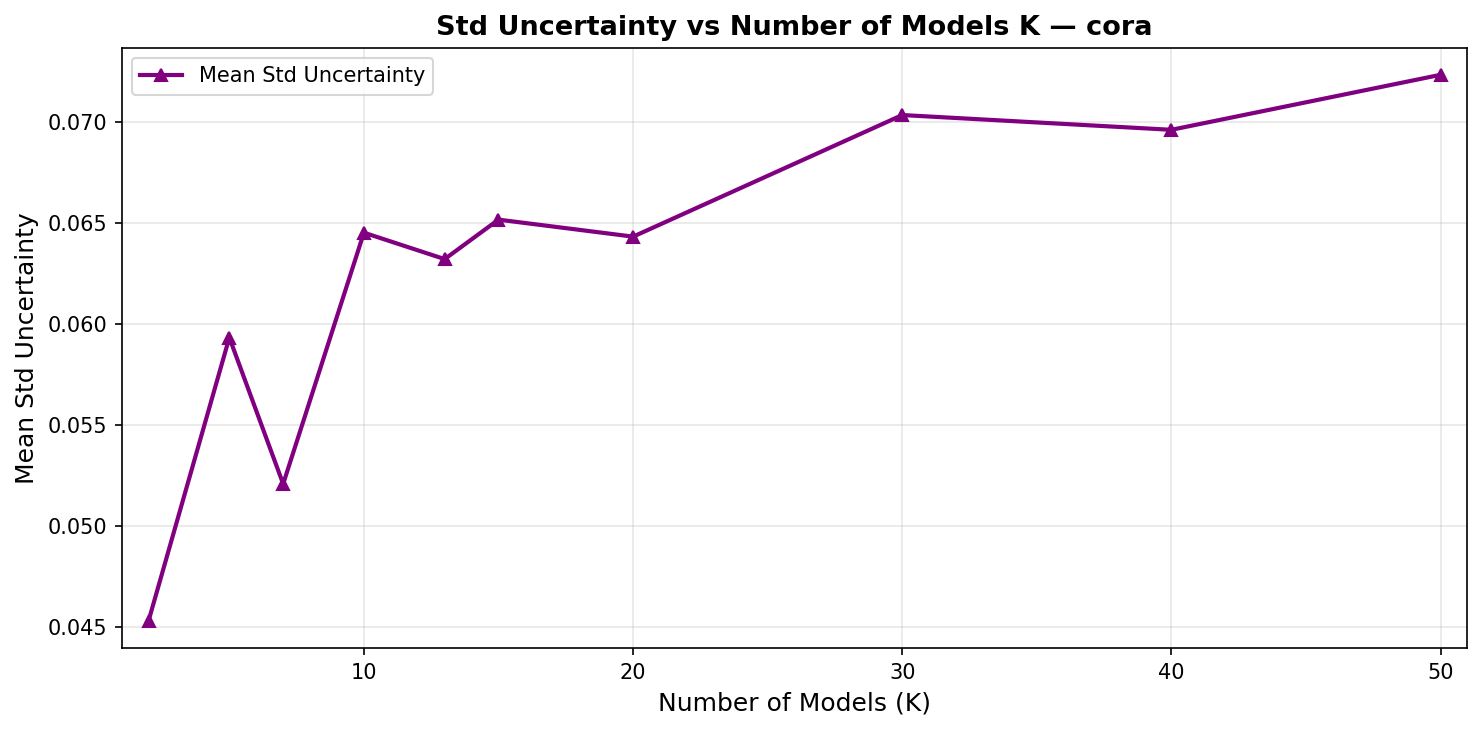
\includegraphics[width=0.5\textwidth]{Images/std_uncertainty_vs_K_cora.png}
\caption{Effect of the number of edge prediction models on the average uncertainty based on the standard deviation measure}
    \label{fig:std_uncertainty_vs_K_cora}
\end{figure}

\begin{figure}[h]
    \centering
    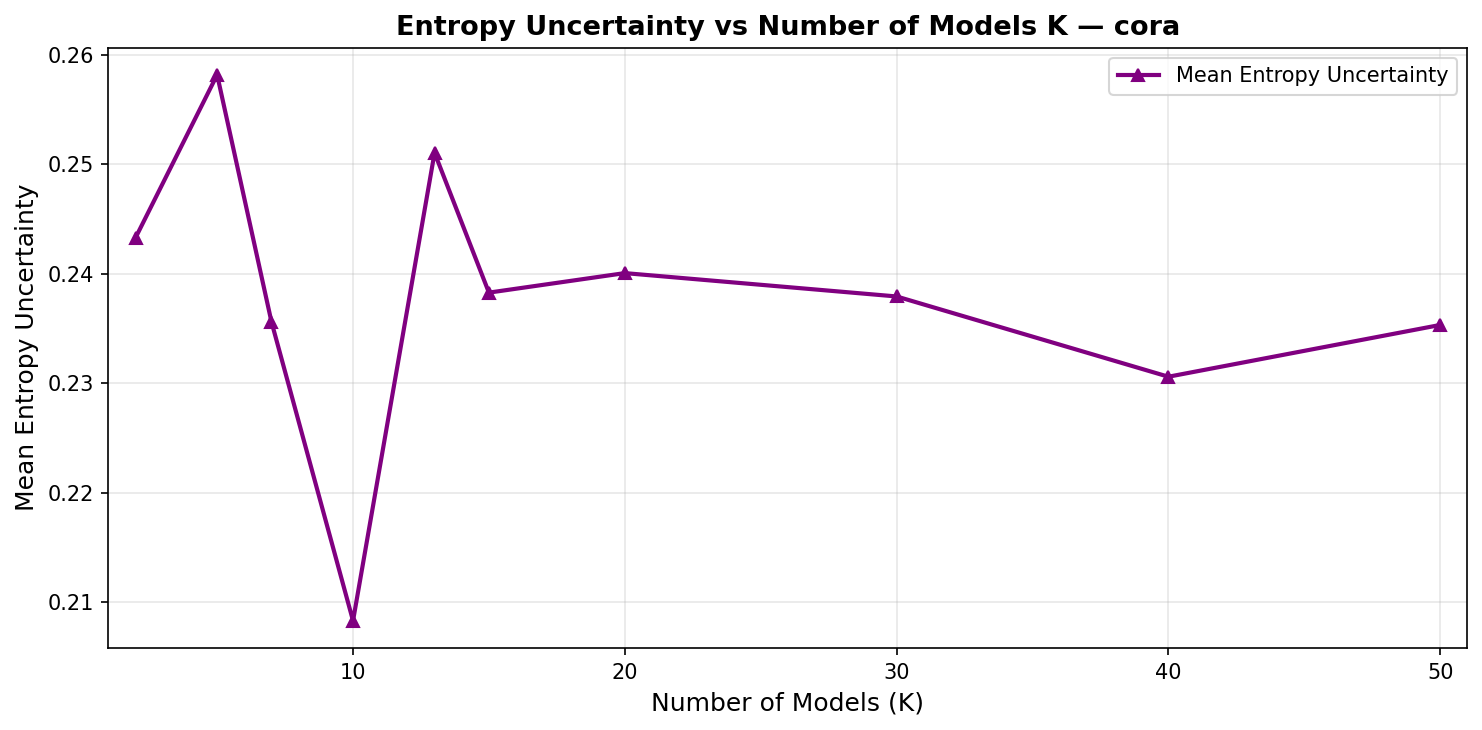
\includegraphics[width=0.5\textwidth]{Images/entropy_uncertainty_vs_K_cora.png}
\caption{Effect of the number of edge prediction models on the average uncertainty based on the entropy measure}
    \label{fig:entropy_uncertainty_vs_K_cora}
\end{figure}

\begin{figure}[h]
    \centering
    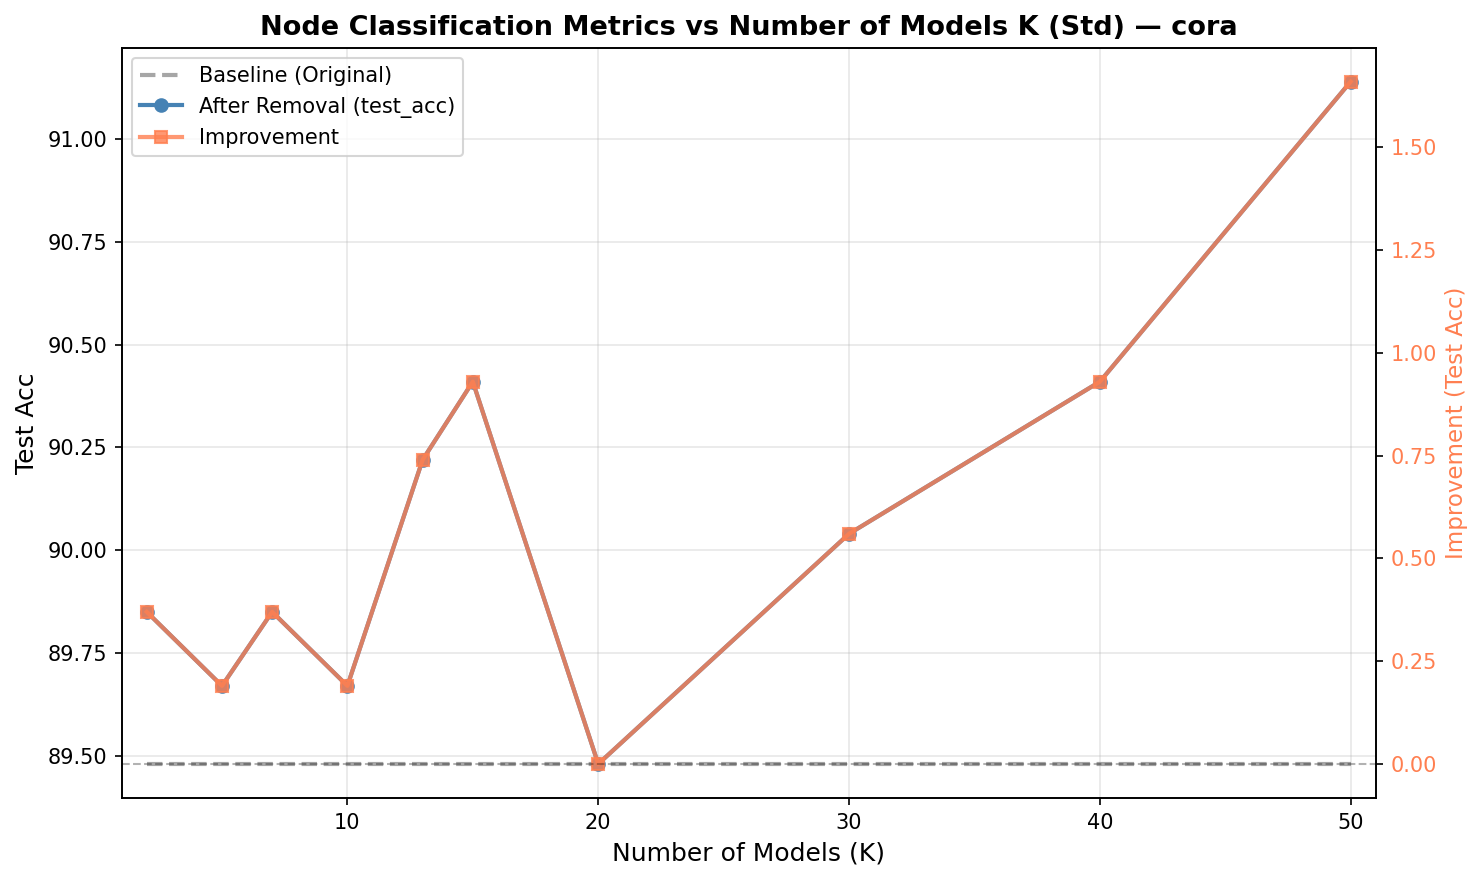
\includegraphics[width=0.5\textwidth]{Images/line_plot_combined_testacc_std_num_models_cora.png}
\caption{
Effect of the number of edge prediction models on graph model performance
in node classification using the standard deviation uncertainty measure
}
    \label{fig:line_plot_combined_testacc_std_num_models_cora}
\end{figure}

\begin{figure}[h]
    \centering
    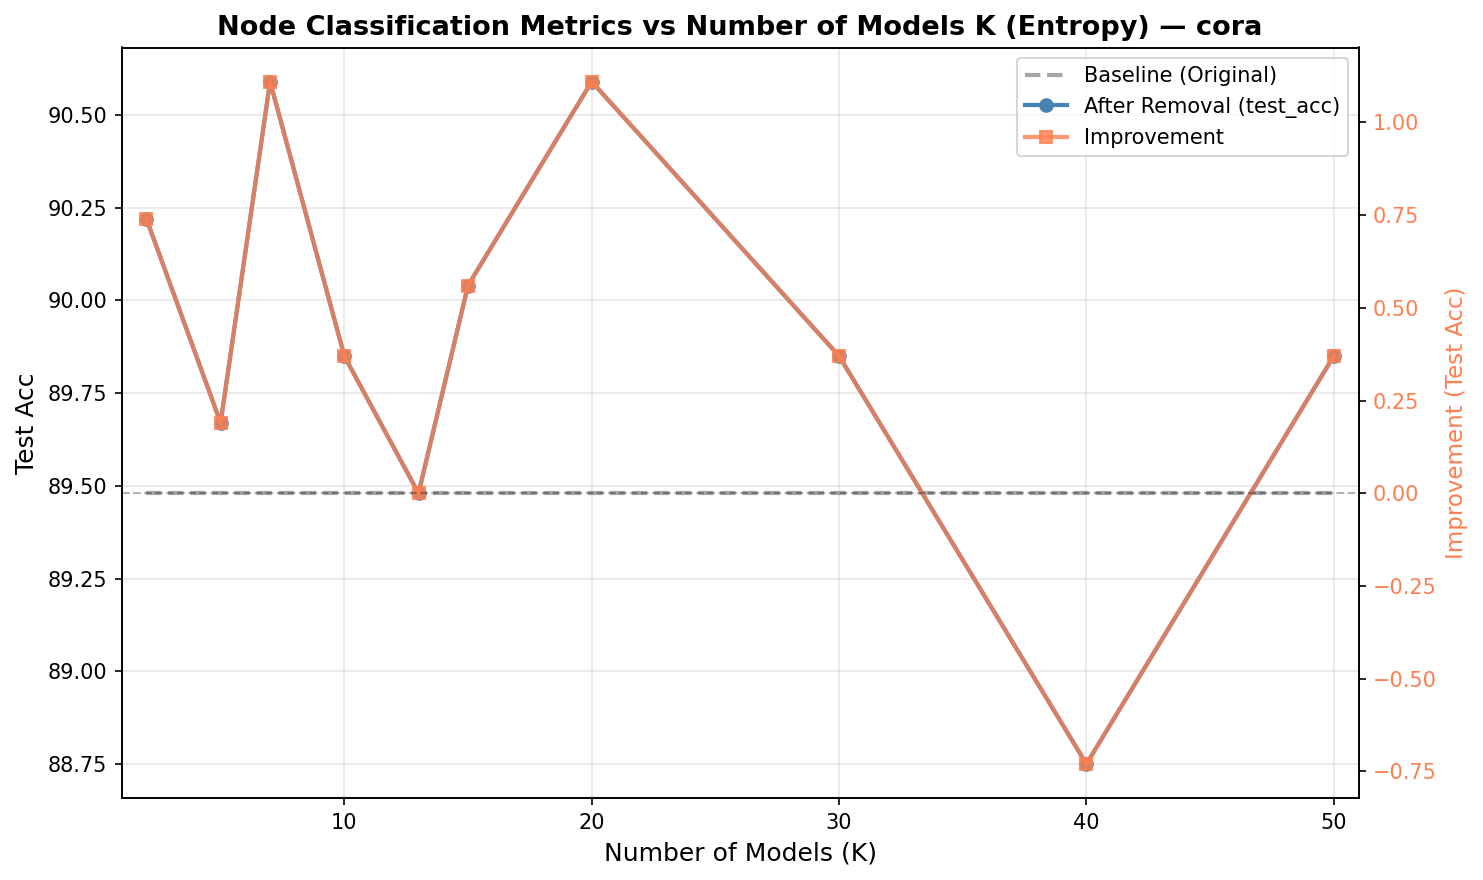
\includegraphics[width=0.5\textwidth]{Images/line_plot_combined_testacc_entropy_num_models_cora.png}
\caption{Chapter6
Effect of the number of edge prediction models on graph model performance
in node classification using the entropy uncertainty measure
}
    \label{fig:line_plot_combined_testacc_entropy_num_models_cora}
\end{figure}

In the above plots, the effect of the number of models on the average of two uncertainty measures—
entropy in Figure \ref{fig:entropy_uncertainty_vs_K_cora}
and standard deviation in Figure \ref{fig:std_uncertainty_vs_K_cora}—
is investigated.

As expected, by increasing the number of edge prediction models,
the uncertainty estimation becomes more stable,
since predictions are averaged and random fluctuations are reduced.
However, increasing the number of generated predictions
can also lead to greater dispersion of values,
thereby increasing the standard deviation.

For the entropy measure,
as the number of models increases,
the measured uncertainty decreases,
since the distribution of predicted probabilities becomes more concentrated.
As a result, as shown in Figure
\ref{fig:line_plot_combined_testacc_entropy_num_models_cora},
fewer edges are identified and removed as noisy,
and some noisy edges remain in the graph,
which can lead to a drop in model performance.

In contrast, when the standard deviation measure is used
(Figure \ref{fig:line_plot_combined_testacc_std_num_models_cora}),
increasing the number of models
enhances sensitivity to prediction fluctuations,
leading to more accurate identification and removal of noisy edges,
and ultimately improving the final model performance.

\subsection{Comparison of Two Structural Refinement Methods with a Random Baseline Model}

\begin{table}[ht]
\centering
\caption{
Comparison of base model accuracy, cosine similarity-based structural refinement,
uncertainty-based refinement (standard deviation and entropy),
and random edge removal
}
\label{tab:compare_structural_enhancer_random_model}
\begin{tabularx}{\linewidth}{c c || *{5}{X}}
\hline
\multirow{2}{*}{Dataset} &
\multirow{2}{*}{Approach} &
\multicolumn{5}{c}{Method} \\
\cline{3-7}
 &  & PiSSA & Orthogonal & EVA & Gaussian & LoFTQ \\
\hline

\multirow{5}{*}{Cora}
 & Base
 & \textbf{90.77} & 89.48 & 92.07 & 91.14 & 90.96 \\
\cline{2-7}
 & Cosine
 & \textbf{90.77} & 90.41 & 92.07 & 90.04 & \textbf{91.88} \\
\cline{2-7}
 & Uncertainty(std)
 & 89.67 & 91.51 & \textbf{92.44} & 91.88 & 91.14 \\
\cline{2-7}
 & Uncertainty(Entropy)
 & 89.48 & \textbf{91.70} & \textbf{92.44} & \textbf{92.25} & 91.51 \\
\cline{2-7}
 & Random
 & 88.56 & 89.59 & 90.88 & 90.14 & 89.41 \\
\hline
\hline

\multirow{5}{*}{PubMed}
 & Base
 & 96.32 & 93.79 & 96.96 & 94.80 & 96.17 \\
\cline{2-7}
 & Cosine
 & \textbf{96.81} & 93.86 & 96.96 & 94.80 & 96.75 \\
\cline{2-7}
 & Uncertainty(std)
 & 96.55 & \textbf{94.17} & \textbf{97.08} & 94.85 & \textbf{96.91} \\
\cline{2-7}
 & Uncertainty(Entropy)
 & 96.50 & 94.07 & 97.06 & \textbf{94.88} & \textbf{96.91} \\
\cline{2-7}
 & Random
 & 93.74 & 90.84 & 91.91 & 90.52 & 93.83 \\
\hline
\hline

\multirow{5}{*}{CiteSeer}
 & Base
 & 80.25 & 80.25 & 79.47 & 81.03 & 80.41 \\
\cline{2-7}
 & Cosine
 & 80.25 & 81.97 & 79.15 & 81.03 & 79.78 \\
\cline{2-7}
 & Uncertainty(std)
 & 81.35 & 82.45 & \textbf{80.72} & \textbf{83.70} & \textbf{81.82} \\
\cline{2-7}
 & Uncertainty(Entropy)
 & \textbf{81.50} & \textbf{83.07} & \textbf{80.72} & 83.54 & 81.66 \\
\cline{2-7}
 & Random
 & 77.62 & 79.56 & 76.68 & 80.19 & 78.94 \\
\hline
\hline

\multirow{5}{*}{WikiCS}
 & Base
 & 87.14 & 85.35 & 87.27 & 86.80 & 87.74 \\
\cline{2-7}
 & Cosine
 & \textbf{88.12} & 85.48 & \textbf{88.64} & 87.01 & \textbf{89.06} \\
\cline{2-7}
 & Uncertainty(std)
 & 87.27 & \textbf{85.73} & 87.40 & 87.01 & 87.83 \\
\cline{2-7}
 & Uncertainty(Entropy)
 & 87.27 & 85.43 & 87.61 & \textbf{87.14} & 88.12 \\
\cline{2-7}
 & Random
 & 84.18 & 82.18 & 85.44 & 82.53 & 81.80 \\
\hline

\end{tabularx}
\end{table}

In this experiment, the goal is to compare the structural enhancement methods introduced in the second and third approaches,
along with a random removal model, against the base model.
The accuracy results of this comparison are presented in Table
\ref{tab:compare_structural_enhancer_random_model}.

In the first row of the table, the performance of the base model without any structural refinement is reported.
In the second row, the results of cosine similarity-based structural refinement (the second method) are presented.
In the third and fourth rows, the results of the third method are reported,
where uncertainty measures are used to detect noisy edges;
specifically, standard deviation is used in the third row
and entropy in the fourth row.
Finally, the fifth row presents the results of the random model,
in which 30\% of edges are randomly removed.

Based on the observed results,
in most datasets the use of cosine similarity in the second method
leads to improved performance compared to the base model.
However, the uncertainty-based method
generally shows more stable and reliable improvements,
indicating its stronger ability to identify noisy edges in a targeted manner.

In some datasets, the second method achieves greater improvements than the third method,
while in others the third method performs better.
This difference suggests that the effectiveness of each method
may depend on structural properties, homophily level,
and the statistical distribution of the data.

On the other hand, the results of the random model show that
non-targeted edge removal leads to a significant drop in performance.
This confirms that the improvements obtained by the proposed methods
are due to systematic and informed removal of noisy edges,
rather than random or uncontrolled deletion.
In other words, in the proposed approaches,
noisy edges are defined and selected in a way that their removal
improves node classification performance.

```latex id="t8v3nc"
\subsection{Single-Representation Ensemble Learning}

\begin{table}[ht]
\centering
\caption{
Comparison of ensemble learning accuracy based on a single representation
on graph-refined structures using standard deviation,
compared to the DIVERGE method
}
\begin{tabularx}{\textwidth}{l||XXXXXX}
\hline
Dataset & PiSSA & EVA & Orthogonal & LoFTQ & Gaussian & DIVERGE \\
\hline
\hline
Cora     & 89.85 & 92.80 & 92.80 & 92.07 & 92.62 & \textbf{93.17} \\
PubMed   & 96.60 & 97.08 & 94.35 & 96.96 & 94.95 & \textbf{97.16} \\
CiteSeer & 79.94 & 78.68 & 78.68 & 79.47 & \textbf{82.60} & 82.13 \\
WikiCS   & 87.27 & 87.40 & 85.65 & 87.87 & 87.23 & \textbf{88.42} \\
\hline
\end{tabularx}
\end{table}

\begin{table}[ht]
\centering
\caption{
Comparison of Macro-F1 scores for ensemble learning based on a single representation
on graph-refined structures using standard deviation,
compared to the DIVERGE method
}
\begin{tabularx}{\textwidth}{l||XXXXXX}
\hline
Dataset & PiSSA & EVA & Orthogonal & LoFTQ & Gaussian & DIVERGE \\
\hline
\hline
Cora     & 87.96 & 91.25 & 91.63 & 90.75 & 90.95 & \textbf{91.85} \\
PubMed   & 96.14 & 96.64 & 93.73 & 96.52 & 94.31 & \textbf{96.75} \\
CiteSeer & 76.29 & 75.13 & 75.13 & 76.71 & \textbf{80.13} & 79.04 \\
WikiCS   & 85.78 & 86.07 & 84.14 & 86.30 & 86.02 & \textbf{87.18} \\
\hline
\end{tabularx}
\end{table}

\begin{table}[ht]
\centering
\caption{
Comparison of ensemble learning accuracy based on a single representation
on graph-refined structures using entropy,
compared to the DIVERGE method
}
\begin{tabularx}{\linewidth}{l||XXXXXX}
\hline
Dataset & PiSSA & EVA & Orthogonal & LoFTQ & Gaussian & DIVERGE \\ 
\hline
\hline
Cora     & 89.11 & 92.44 & 92.07 & 92.07 & 92.62 & \textbf{93.17} \\ 
PubMed   & 96.53 & 97.08 & 94.27 & 96.98 & 94.98 & \textbf{97.16} \\ 
CiteSeer & 80.72 & 79.15 & 78.84 & 79.47 & \textbf{83.07} & 82.13 \\ 
WikiCS   & 87.36 & 87.36 & 85.73 & 88.17 & 87.14 & \textbf{88.42} \\ 
\hline
\end{tabularx}
\end{table}

\begin{table}[ht]
\centering
\caption{
Comparison of Macro-F1 scores for ensemble learning based on a single representation
on graph-refined structures using entropy,
compared to the DIVERGE method
}
\begin{tabularx}{\linewidth}{l||XXXXXX}
\hline
Dataset & PiSSA & EVA & Orthogonal & LoFTQ & Gaussian & DIVERGE \\ 
\hline
\hline
Cora     & 87.01 & 90.69 & 90.53 & 90.65 & 91.25 & \textbf{91.85} \\ 
PubMed   & 96.04 & 96.64 & 93.65 & 96.57 & 94.41 & \textbf{96.75} \\ 
CiteSeer & 77.26 & 76.10 & 76.79 & 76.15 & \textbf{79.99} & 79.04 \\ 
WikiCS   & 85.99 & 86.40 & 84.36 & 86.78 & 85.82 & \textbf{87.18} \\ 
\hline
\end{tabularx}
\end{table}
```

In this experiment, the objective is to investigate the feasibility of using a single representation
for performing ensemble learning on refined graphs,
and to compare its performance with the DIVERGE method.

To this end, a single representation is first extracted from the data.
Then, by tuning the hyperparameters of the structural refinement method
based on two criteria—standard deviation and entropy—
multiple refined graphs are generated.
Among them, five graphs with the best performance
according to the same single representation are selected.
Next, the proposed ensemble learning method is applied
only to these five graphs,
and the final results are reported.

The main goal of this experiment is to examine whether it is possible,
using only a single representation,
to achieve performance close to the first method
(based on multiple independent representations) or not.
If this goal is achieved,
a significant reduction in computational time and memory usage can be obtained,
since there is no need to generate and store multiple separate representations.

Based on the observed results,
the performance of the single-representation-based method
is very close to the DIVERGE method in most datasets,
although it is usually slightly lower.
However, in some datasets such as CiteSeer,
the single-representation-based method even achieves better performance.
Overall, these results indicate that under time and memory constraints,
single-representation ensemble learning
can serve as an efficient and cost-effective alternative,
with only a negligible drop in performance.

```latex id="u2k9fd"
\subsection{Comparison of the Two Previous Methods}

\begin{table}[ht]
\centering
\caption{Comparison of accuracy for ensemble learning results using cosine similarity-based structural refinement and uncertainty-based refinement with entropy and standard deviation measures}
\label{tab:accuracy_ensemble_after_enhancers}
\begin{tabularx}{\linewidth}{c c || *{3}{X}}
\hline
Dataset &
Approach &
\multicolumn{3}{c}{Method} \\
\cline{3-5}
 &  & Ensemble 1 & Ensemble 2 & Ensemble 3 \\
\hline

\multirow{4}{*}{Cora}
 & DIVERGE
 & 93.17 & 93.36 & 93.17 \\
\cline{2-5}
 & DIVERGE + cosine
 & \textbf{93.91} & \textbf{94.10} & \textbf{94.10} \\
\cline{2-5}
 & DIVERGE + Uncertainty(std)
 & 93.17 & 93.17 & 93.17 \\
\cline{2-5}
 & DIVERGE + Uncertainty(Entropy)
 & 92.99 & 92.80 & 92.62 \\
\hline
\hline

\multirow{4}{*}{PubMed}
 & DIVERGE
 & 96.98 & 97.13 & 97.16 \\
\cline{2-5}
 & DIVERGE + cosine
 & 97.03 & 97.11 & 97.13 \\
\cline{2-5}
 & DIVERGE + Uncertainty(std)
 & \textbf{97.26} & \textbf{97.16} & \textbf{97.16} \\
\cline{2-5}
 & DIVERGE + Uncertainty(Entropy)
 & 97.13 & 97.11 & 97.13 \\
\hline
\hline

\multirow{4}{*}{CiteSeer}
 & DIVERGE
 & 81.66 & 81.97 & 82.13 \\
\cline{2-5}
 & DIVERGE + cosine
 & 81.03 & 81.82 & 81.50 \\
\cline{2-5}
 & DIVERGE + Uncertainty(std)
 & 81.82 & 82.29 & 81.66 \\
\cline{2-5}
 & DIVERGE + Uncertainty(Entropy)
 & \textbf{83.07} & \textbf{82.76} & \textbf{82.92} \\
\hline
\hline

\multirow{4}{*}{WikiCS}
 & DIVERGE
 & 88.34 & 88.38 & 88.42 \\
\cline{2-5}
 & DIVERGE + cosine
 & \textbf{89.32} & \textbf{89.19} & \textbf{89.28} \\
\cline{2-5}
 & DIVERGE + Uncertainty(std)
 & 88.30 & 88.38 & 88.59 \\
\cline{2-5}
 & DIVERGE + Uncertainty(Entropy)
 & 88.64 & 88.51 & 88.64 \\
\hline

\end{tabularx}
\end{table}

\begin{table}[ht]
\centering
\caption{Comparison of Macro-F1 results for ensemble learning using cosine similarity-based structural refinement and uncertainty-based refinement with entropy and standard deviation measures}
\label{tab:macro_f1_ensemble_after_enhancers}
\begin{tabularx}{\linewidth}{c c || *{3}{X}}
\hline
Dataset &
Approach &
\multicolumn{3}{c}{Method} \\
\cline{3-5}
 &  & Ensemble 1 & Ensemble 2 & Ensemble 3 \\
\hline

\multirow{4}{*}{Cora}
 & DIVERGE & 92.06 & 91.80 & 91.85 \\
\cline{2-5}
 & DIVERGE + cosine & \textbf{92.65} & \textbf{92.99} & \textbf{92.96} \\
\cline{2-5}
 & DIVERGE + Uncertainty(std) & 91.96 & 91.96 & 91.96 \\
\cline{2-5}
 & DIVERGE + Uncertainty(Entropy) & 91.77 & 91.43 & 91.59 \\
\hline
\hline

\multirow{4}{*}{PubMed}
 & DIVERGE & 96.56 & 96.74 & 96.75 \\
\cline{2-5}
 & DIVERGE + cosine & 96.60 & 96.74 & 96.77 \\
\cline{2-5}
 & DIVERGE + Uncertainty(std) & \textbf{96.88} & \textbf{96.79} & \textbf{96.78} \\
\cline{2-5}
 & DIVERGE + Uncertainty(Entropy) & 96.70 & 96.73 & 96.74 \\
\hline
\hline

\multirow{4}{*}{CiteSeer}
 & DIVERGE & 79.25 & 78.83 & 79.04 \\
\cline{2-5}
 & DIVERGE + cosine & 77.92 & 78.56 & 78.37 \\
\cline{2-5}
 & DIVERGE + Uncertainty(std) & 79.30 & 79.79 & 78.41 \\
\cline{2-5}
 & DIVERGE + Uncertainty(Entropy) & \textbf{79.37} & \textbf{79.54} & \textbf{79.50} \\
\hline
\hline

\multirow{4}{*}{WikiCS}
 & DIVERGE & 86.96 & 87.03 & 87.18 \\
\cline{2-5}
 & DIVERGE + cosine & \textbf{88.43} & \textbf{88.27} & \textbf{88.09} \\
\cline{2-5}
 & DIVERGE + Uncertainty(std) & 87.09 & 87.10 & 87.41 \\
\cline{2-5}
 & DIVERGE + Uncertainty(Entropy) & 87.61 & 87.38 & 87.51 \\
\hline
\end{tabularx}
\end{table}
```

In the two presented tables, the accuracy metrics
(\ref{tab:accuracy_ensemble_after_enhancers})
and Macro-F1
(\ref{tab:macro_f1_ensemble_after_enhancers})
are compared for the DIVERGE method with and without structural refinement.

In the first row, the results of DIVERGE without any structural refinement are reported.
In the second row, the results of DIVERGE after applying cosine similarity–based refinement are presented.
In the third and fourth rows, the results of DIVERGE after uncertainty-based refinement are reported; where, in the third row, the standard deviation criterion is used, and in the fourth row, entropy is used for identifying noisy edges. The table columns correspond to the three ensemble learning methods introduced within the DIVERGE framework.

The comparison shows that, in most datasets, applying structural refinement prior to ensemble learning leads to improved performance. This finding indicates that the targeted removal of noisy edges can improve graph structure quality and enhance message passing in graph neural networks.

It is also observed that the two structural refinement approaches (cosine similarity–based and uncertainty-based) exhibit competitive and complementary behavior. In some datasets, cosine-based refinement yields better results, while in others, uncertainty-based refinement performs better. This suggests that the effectiveness of each method depends on the structural and statistical properties of the graph, and neither approach is strictly dominant.


\section{Results}

\bibliographystyle{plainnat}
\bibliography{references}


\end{document}

